\documentclass[../main.tex]{subfiles}
Este capítulo presenta los resultados obtenidos sobre el software desarrollado. En primer lugar, se muestra un manual de usuario sobre la aplicación. Este manual realiza un viaje gráfico por cada una de las ventanas y pestañas mostrando cada una de las funciones de la aplicación. \\
En según lugar, se recogen en forma de casos de uso diferentes acciones típicas que se pueden realizar con la aplicación. El motivo de los casos de uso es ejemplificar y poner en práctica lo explicado durante el manual de usuario. Un caso de uso trata de mostrar al lector la secuencia de acciones a realizar para completar una tarea. Suponen pues una especie de guía de aprendizaje de la aplicación. El lector tiene que ser consciente que no se representan todas las acciones disponibles en la aplicación, sino las más comunes en un uso estándar. Existirán acciones que sin estar especificadas en los casos de uso se podrán realizar según lo mostrado en el manual de usuario. 

\section{Manual de Usuario}
El manual de usuario se divide en tres diferentes secciones. Se distingue entre menús, ventana principal y ventanas secundarias. Para cada una de estas secciones y sus sucesivas secciones internas se muestra una captura de pantalla junto con una tabla que expone las diferentes opciones disponibles y una breve explicación de la misma. Esta sección imita el formato la sencillez y brevedad de un manual de usuario, donde la escasez de texto es una virtud.

\clearpage

\subsection{Menús} \label{subsection:man-menu}
La aplicación solo dispone de un menú, el menú de fichero (Secc. \ref{subsubsection:man-fich}).

\subsubsection{Menú de Fichero} \label{subsubsection:man-fich}
El menú de fichero \emph{File} dispone de dos acciones, de configuración y de salida. La acción de configuración permite cambiar el origen del mapa mostrado en la escena y abrir la ventana secundaria de configuración (Secc. \ref{subsubsection:man-config}).

\begin{figure}[H]
    \centering
    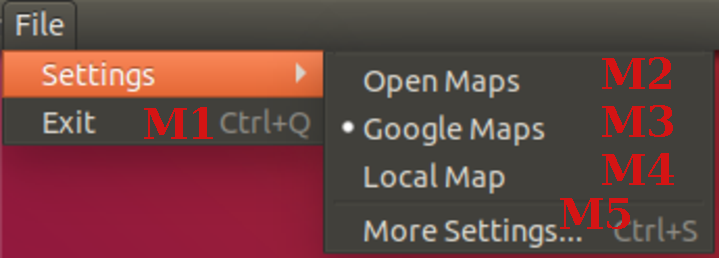
\includegraphics[width=0.5\textwidth]{man/menu.pdf}
\end{figure}

\begin{table}[H]
    \centering
    \begin{threeparttable}
        \begin{tabular}{| l | l |}
            \hline
            \thead{Nº} & \thead{Descripción} \\ \hline
            
            M1 & Opción para cerrar la aplicación. \\ \hline
            M2 & Opción de cambio de escena a mapas abiertos. \\ \hline
            M3 & Opción de cambio de escena a mapas de Google. \\ \hline
            M4 & Opción de cambio de escena a mapas locales. \\ \hline
            M5 & Opción para abrir ventana de configuración (Ver \ref{subsubsection:man-config}). \\ \hline
        \end{tabular}
        
    \end{threeparttable}
\end{table}

\clearpage

\subsection{Ventana Principal} \label{subsection:man-vent-princ}
Dentro de la ventana principal de la aplicación se distinguen el panel de navegación (Secc. \ref{subsubsection:man-naveg}) y las cinco pestañas disponibles; \emph{Setup} (Secc. \ref{subsubsection:man-setup}), \emph{Mission} (Secc. \ref{subsubsection:man-mission}), \emph{Checklist} (Secc. \ref{subsubsection:man-check}), \emph{Follow} (Secc. \ref{subsubsection:man-follow}) y \emph{Log} (Secc. \ref{subsubsection:man-log}).

\subsubsection{Panel de Navegación} \label{subsubsection:man-naveg}
El panel de navegación permite fundamentalmente la navegación entre las diferentes pestañas de la aplicación y el establecimiento/cierre de la conexión con la aeronave. 

\begin{figure}[H]
    \centering
    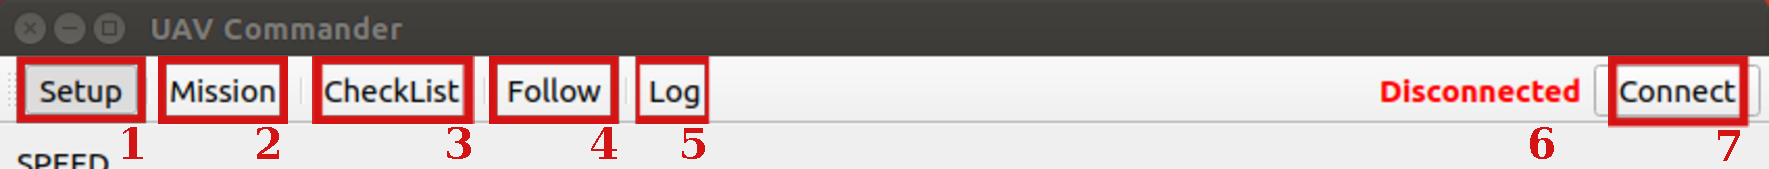
\includegraphics[width=\textwidth]{man/navegacion.pdf}
\end{figure}

\begin{table}[H]
    \centering
    \begin{threeparttable}
        \begin{tabular}{| l | l |}
            \hline
            \thead{Nº} & \thead{Descripción} \\ \hline
            
            1 & Botón para acceder a la pestaña \emph{Setup} (Ver \ref{subsubsection:man-setup}). \\ \hline
            2 & Botón para acceder a la pestaña \emph{Mission} (Ver \ref{subsubsection:man-mission}). \\ \hline
            3 & Botón para acceder a la pestaña \emph{Checklist} (Ver \ref{subsubsection:man-check}). \\ \hline
            4 & Botón para acceder a la pestaña \emph{Follow} (Ver \ref{subsubsection:man-follow}). \\ \hline
            5 & Botón para acceder a la pestaña \emph{Log} (Ver \ref{subsubsection:man-log}). \\ \hline
            6 & Etiqueta que muestra el estado de la conexión. \\ \hline
            7 & Botón para establecer/cortar la conexión. \\ \hline
        \end{tabular}
        
    \end{threeparttable}
\end{table}

\clearpage

\subsubsection{Pestaña \emph{Setup}} \label{subsubsection:man-setup}
La pestaña de \emph{Setup} reúne las acciones de caracterización de la aeronave y su carga de pago.

\begin{figure}[H]
    \centering
    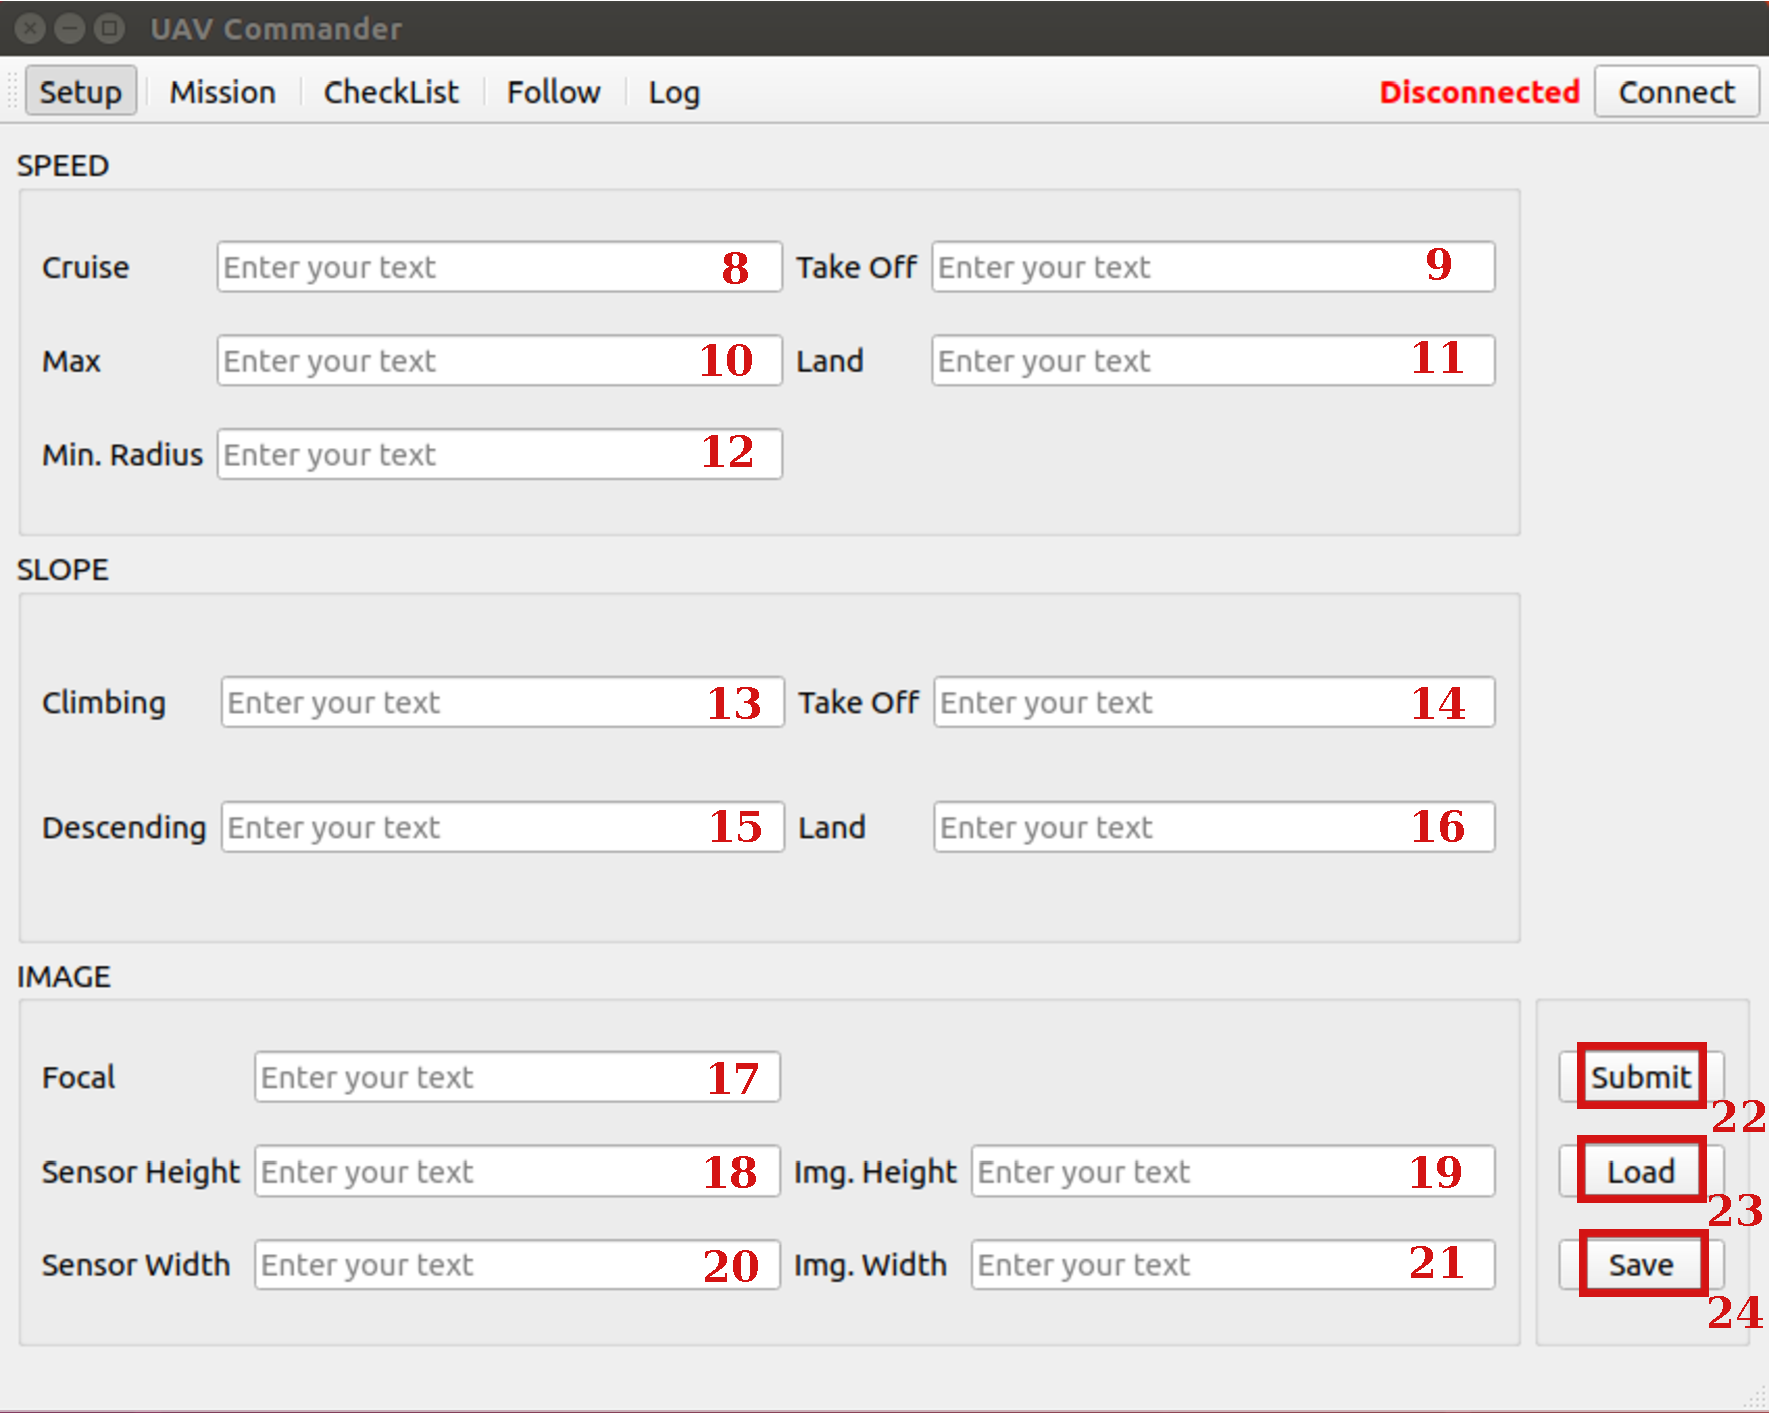
\includegraphics[width=0.9\textwidth]{man/setup.pdf}
\end{figure}

\begin{table}[H]
    \centering
    \begin{threeparttable}
        \begin{tabular}{| l | l |}
            \hline
            \thead{Nº} & \thead{Descripción} \\ \hline
            
            8  & Velocidad de crucero (m/s). \\ \hline
            9  & Velocidad de despegue (m/s). \\ \hline
            10 & Velocidad máxima (m/s). \\ \hline
            11 & Velocidad de aterrizaje (m/s). \\ \hline
            12 & Radio mínimo de giro (m). \\ \hline
            13 & Pendiente de ascenso (º). \\ \hline
            14 & Pendiente de despegue (º). \\ \hline
            15 & Pendiente de descenso (º). \\ \hline
            16 & Pendiente de aterrizaje (º). \\ \hline
            17 & Distancia focal del sensor (mm). \\ \hline
            18 & Alto del sensor (mm). \\ \hline
            19 & Alto de la imagen (px). \\ \hline
            20 & Ancho del sensor (mm). \\ \hline
            21 & Ancho de la imagen (px). \\ \hline
            22 & Botón crear la configuración. \\ \hline
            23 & Botón para cargar una configuración. \\ \hline
            24 & Botón para guardar la configuración. \\ \hline
        \end{tabular}
        
    \end{threeparttable}
\end{table}

\clearpage

\subsubsection{Pestaña \emph{Mission}} \label{subsubsection:man-mission}
La pestaña de \emph{Missión} permite la creación de misiones. Dispone de una escena donde se muestra el mapa y de una serie de herramientas de creación de misión. Sobre esta pestaña se puede acceder al creador de misiones polilínea (Secc. \ref{subsubsubsection:man-pol}) y al creador de misiones por patrón (Secc. \ref{subsubsubsection:man-patron}).

\begin{figure}[H]
    \centering
    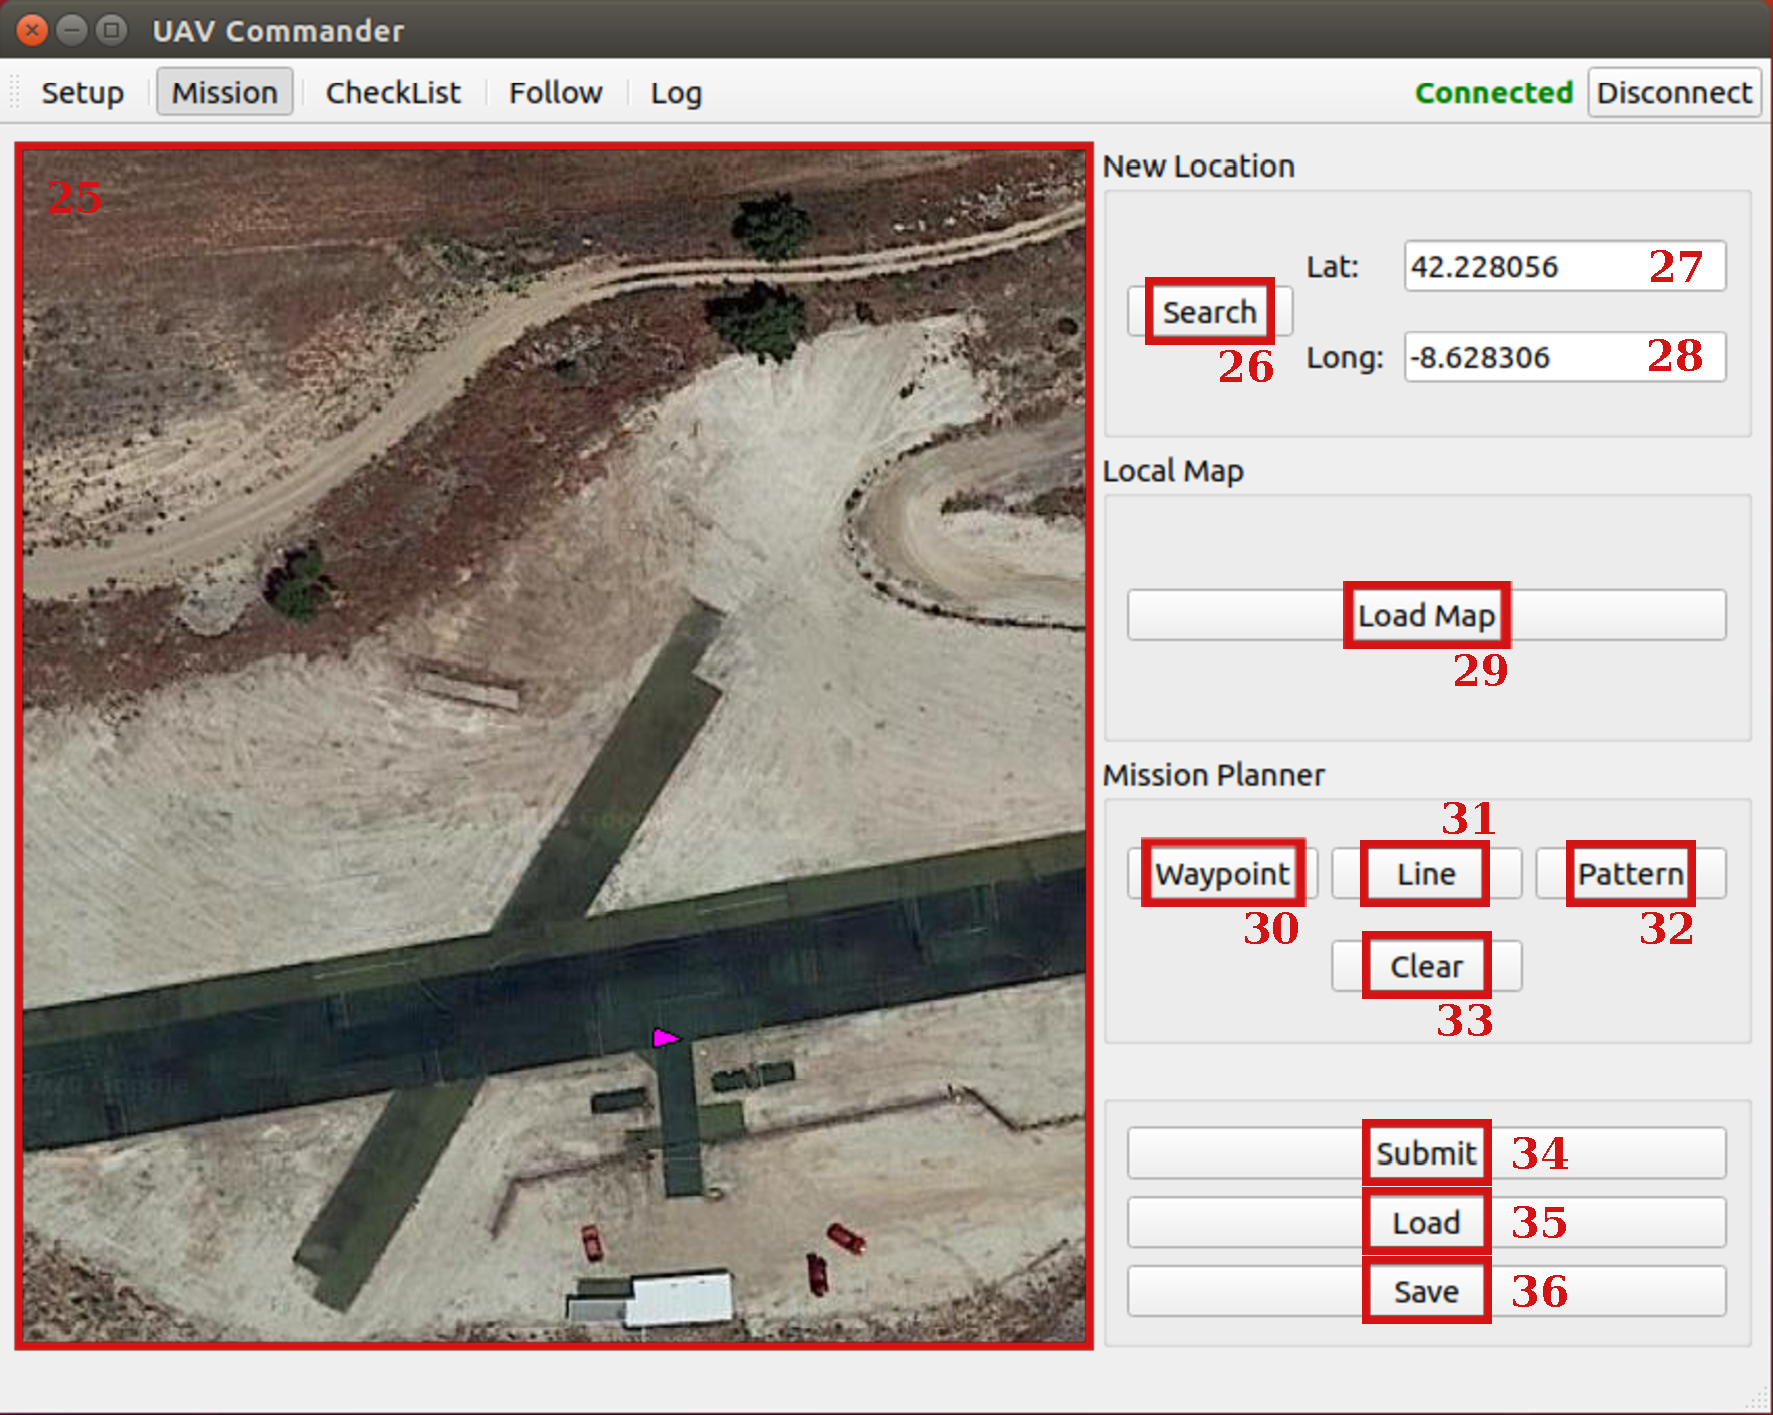
\includegraphics[width=\textwidth]{man/mission.pdf}
\end{figure}

\begin{table}[H]
    \centering
    \begin{threeparttable}
        \begin{tabular}{| l | l |}
            \hline
            \thead{Nº} & \thead{Descripción} \\ \hline
            
            25 & Escena con el mapa cargado. \\ \hline
            26 & Botón para buscar determinada posición en el mapa. \\ \hline
            27 & Latitud (º). \\ \hline
            28 & Longitud (º). \\ \hline
            29 & Botón de carga de mapa local. \\ \hline
            30 & Botón para acceder al creador de misiones multilínea (Ver \ref{subsubsubsection:man-pol}). \\ \hline
            31 & No disponible. \\ \hline
            32 & Botón para acceder al creador de misiones por patrón (Ver \ref{subsubsubsection:man-patron}). \\ \hline
            33 & Botón para borrar la misión activa. \\ \hline
            34 & Botón para crear la misión. \\ \hline
            35 & Botón para cargar una misión. \\ \hline
            36 & Botón para guardar la misión. \\ \hline
        \end{tabular}
        
    \end{threeparttable}
\end{table}

\clearpage

% sub
\subsubsection{Creador de misiones polilínea} \label{subsubsubsection:man-pol}
Para acceder al creador de misiones polilínea es necesario tener pulsada la acción 30 en la pestaña \emph{Mission}.

\begin{figure}[H]
    \centering
    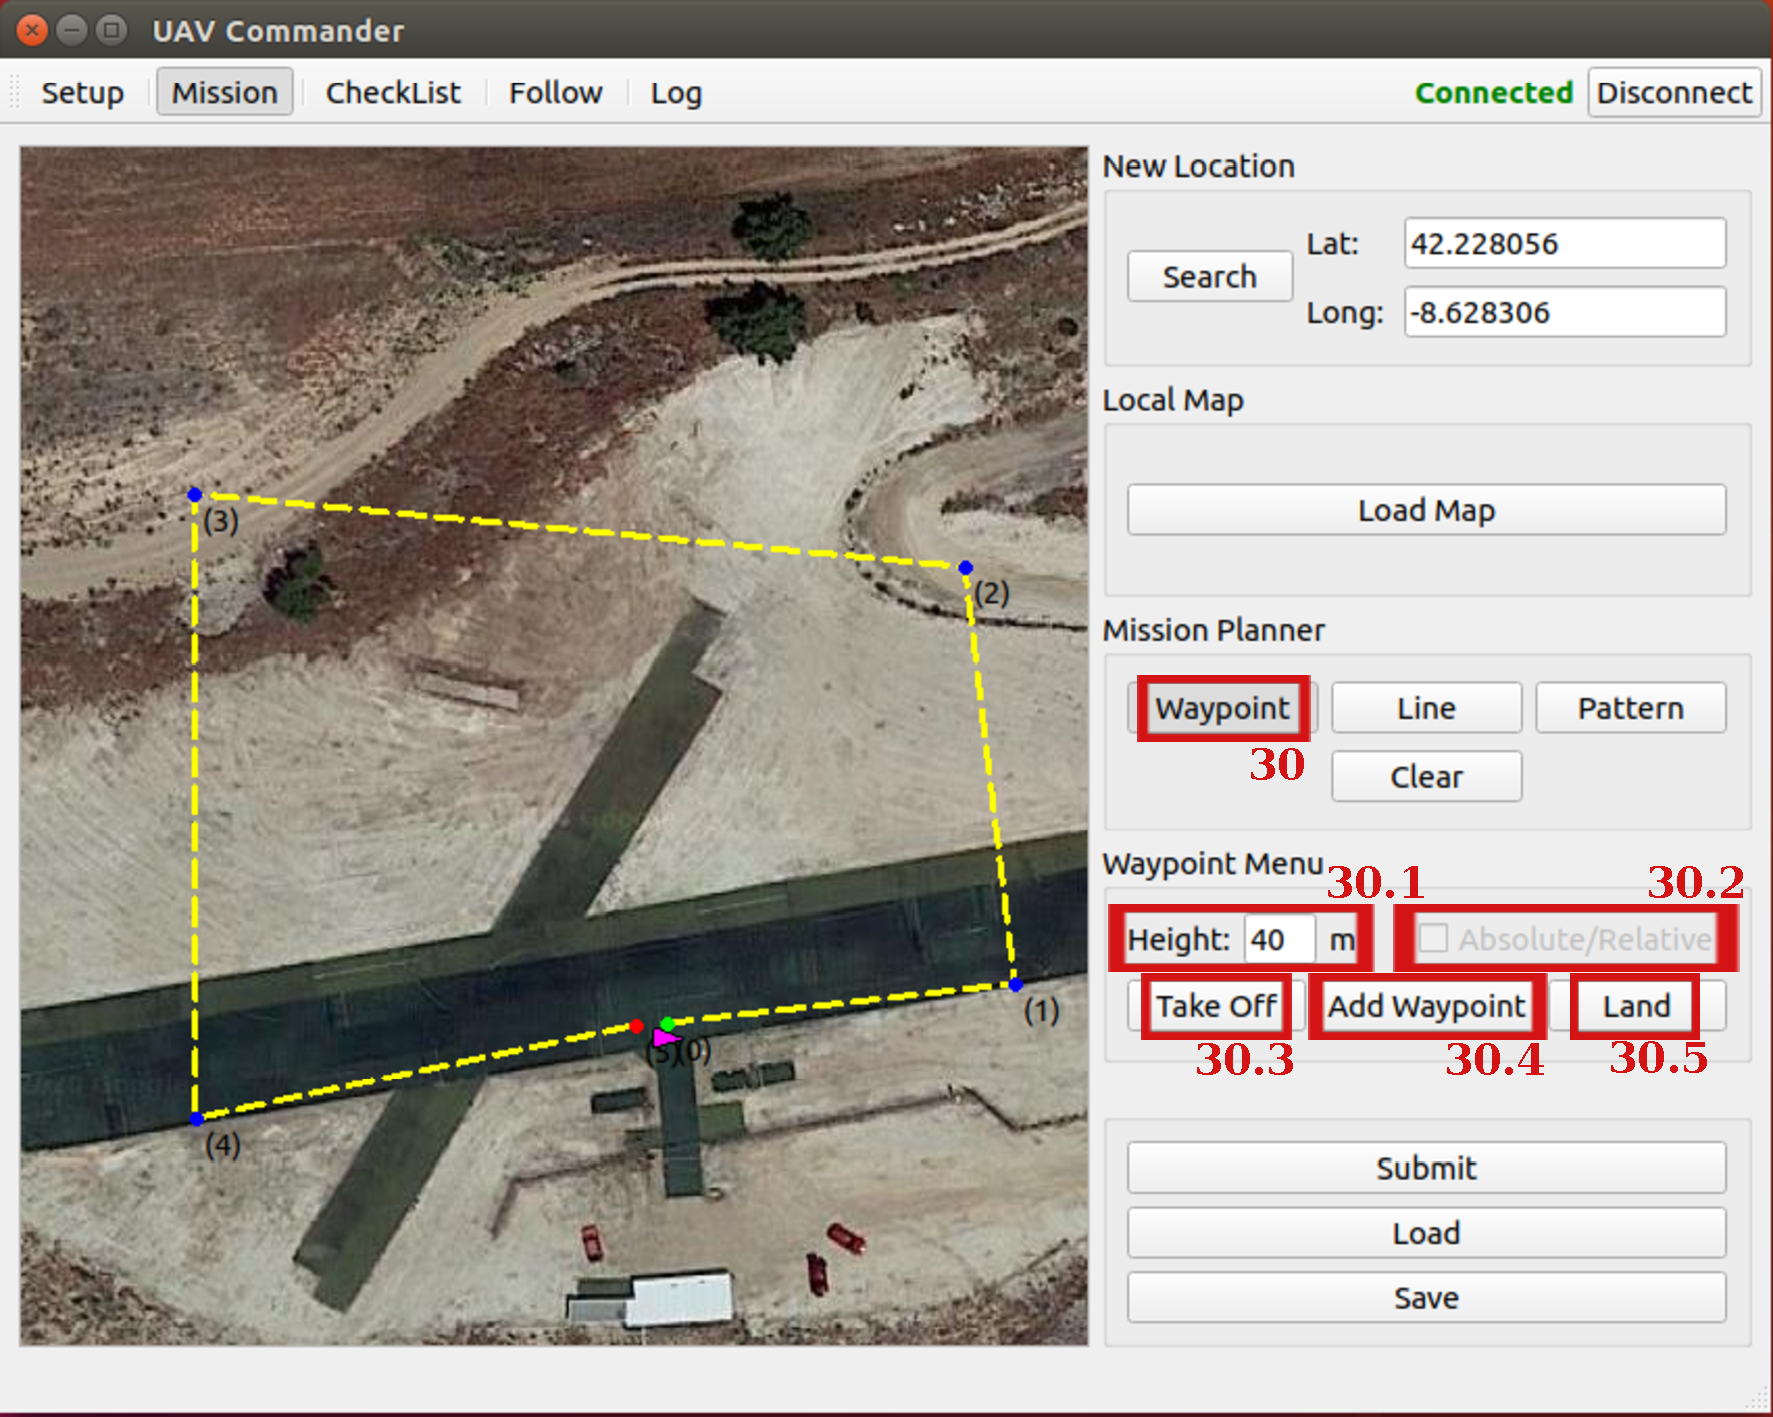
\includegraphics[width=\textwidth]{man/mission-wayp.pdf}
\end{figure}

\begin{table}[H]
    \centering
    \begin{threeparttable}
        \begin{tabular}{| l | l |}
            \hline
            \thead{Nº} & \thead{Descripción} \\ \hline
            
            30.1 & Altura (m). \\ \hline
            30.2 & Altura absoluta o relativa. \\ \hline
            30.3 & Botón para añadir punto de despegue. \\ \hline
            30.4 & Botón para abrir ventana de puntos de paso (Ver \ref{subsubsection:man-puntos}). \\ \hline
            30.5 & Botón para añadir punto de aterrizaje. \\ \hline
        \end{tabular}
        
    \end{threeparttable}
\end{table}

\clearpage

% sub
\subsubsection{Creador de misiones por patrón} \label{subsubsubsection:man-patron}
Para acceder al creador de misiones por patrón es necesario tener pulsada la acción 32 en la pestaña \emph{Mission}.

\begin{figure}[H]
    \centering
    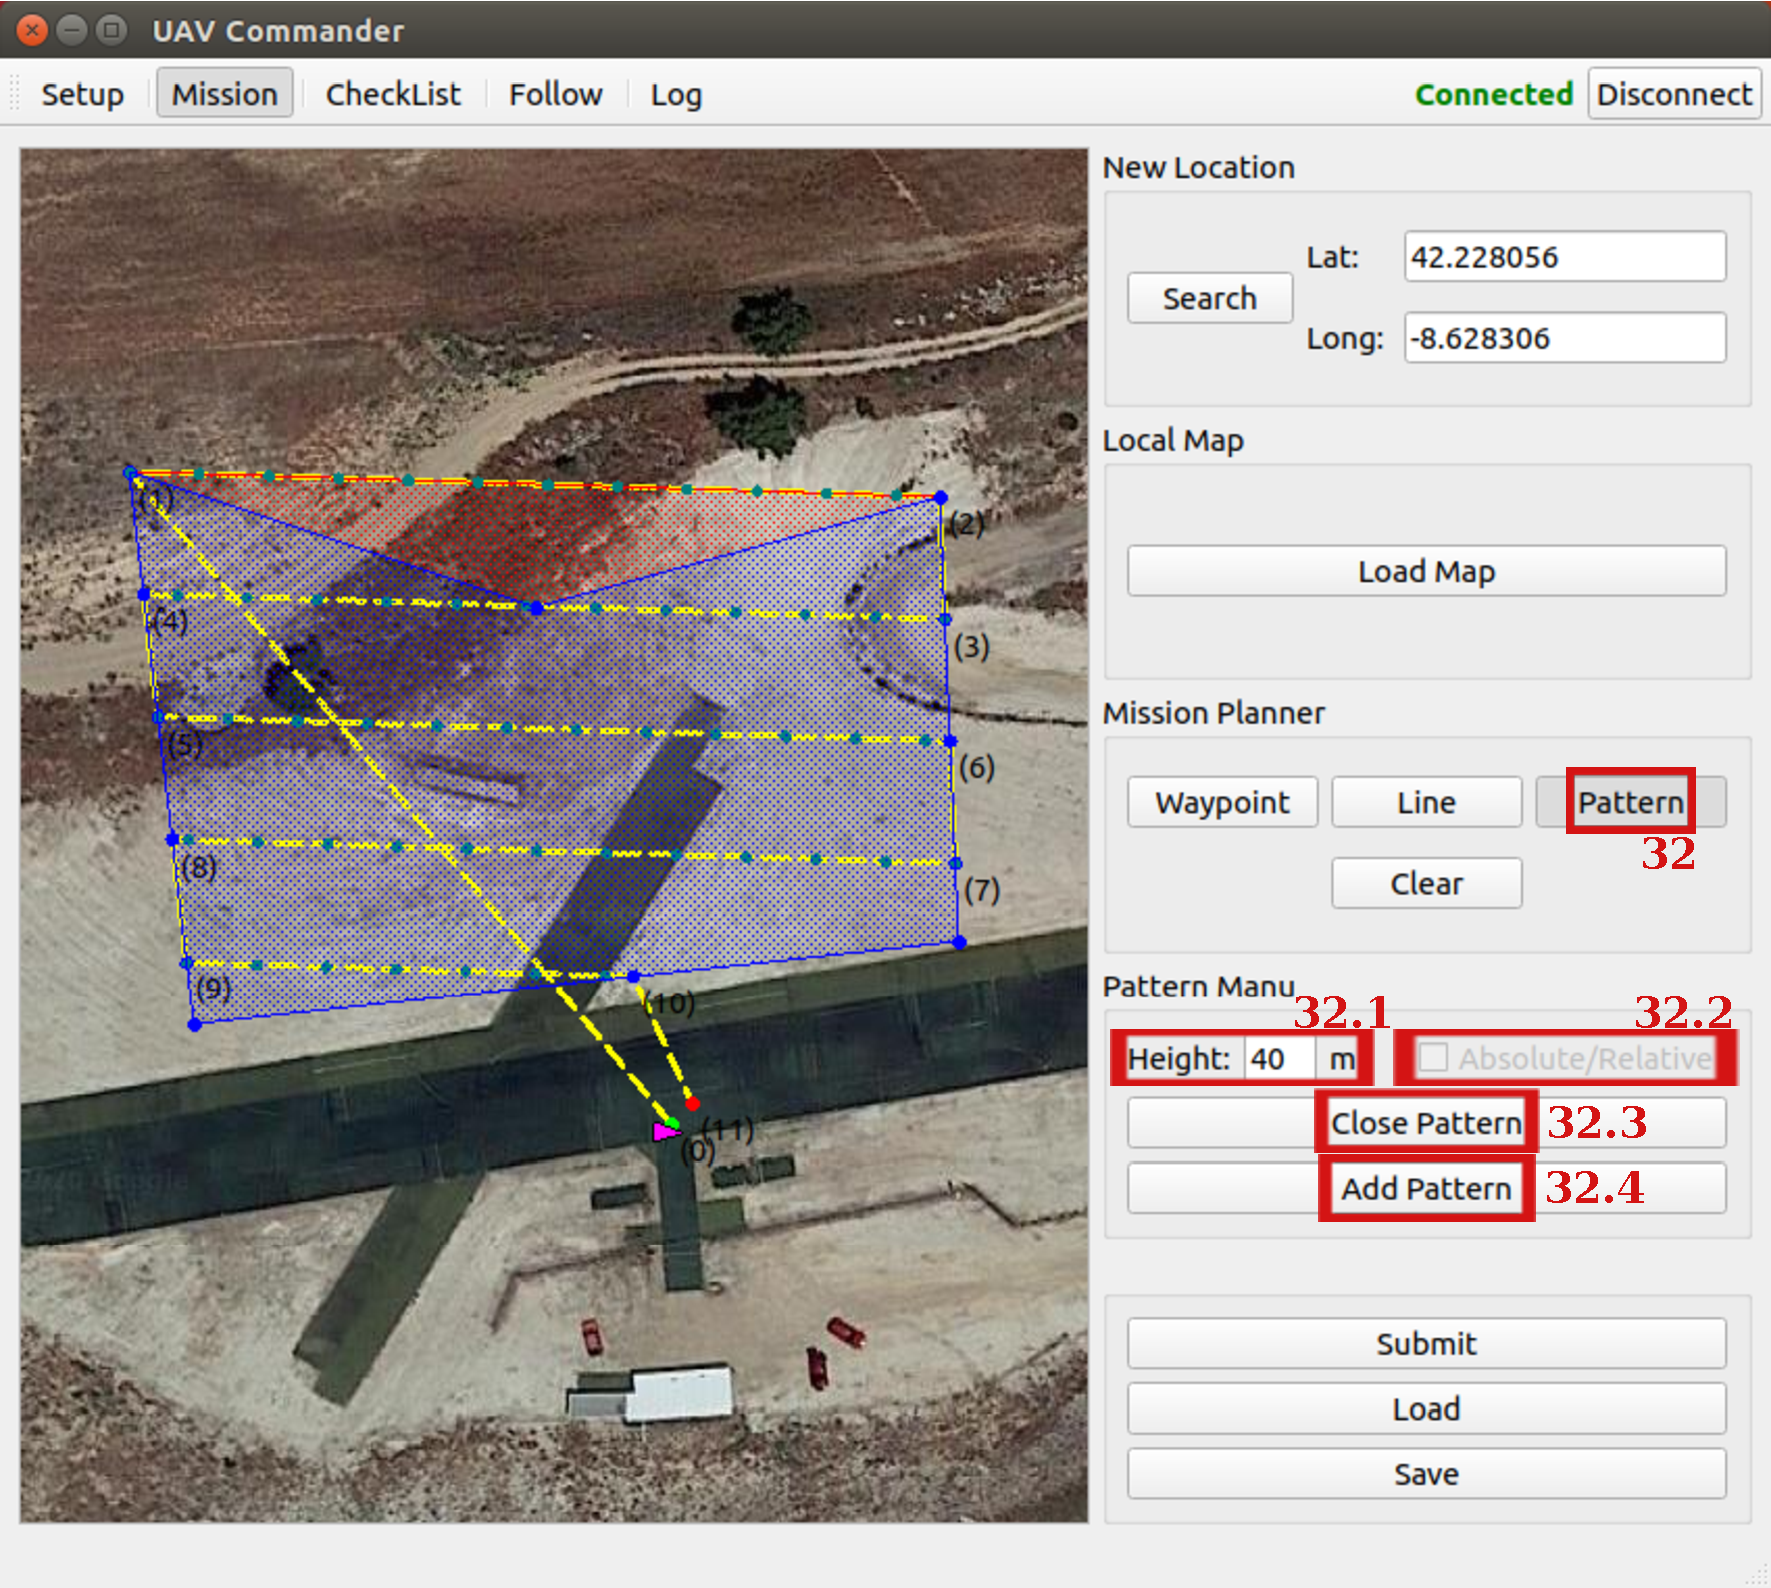
\includegraphics[width=\textwidth]{man/mission-pattern.pdf}
\end{figure}

\begin{table}[H]
    \centering
    \begin{threeparttable}
        \begin{tabular}{| l | l |}
            \hline
            \thead{Nº} & \thead{Descripción} \\ \hline
            
            32.1 & Altura (m). \\ \hline
            32.2 & Altura absoluta o relativa. \\ \hline
            32.3 & Botón para cerrar el patrón. \\ \hline
            32.4 & Botón para abrir ventana de vértices (Ver \ref{subsubsection:man-puntos}). \\ \hline
        \end{tabular}
        
    \end{threeparttable}
\end{table}

\clearpage

\subsubsection{Pestaña \emph{Checklist}} \label{subsubsection:man-check}
La pestaña \emph{Checklist} recoge las comprobaciones pre-vuelo necesarias para poder iniciar una misión.

\begin{figure}[H]
    \centering
    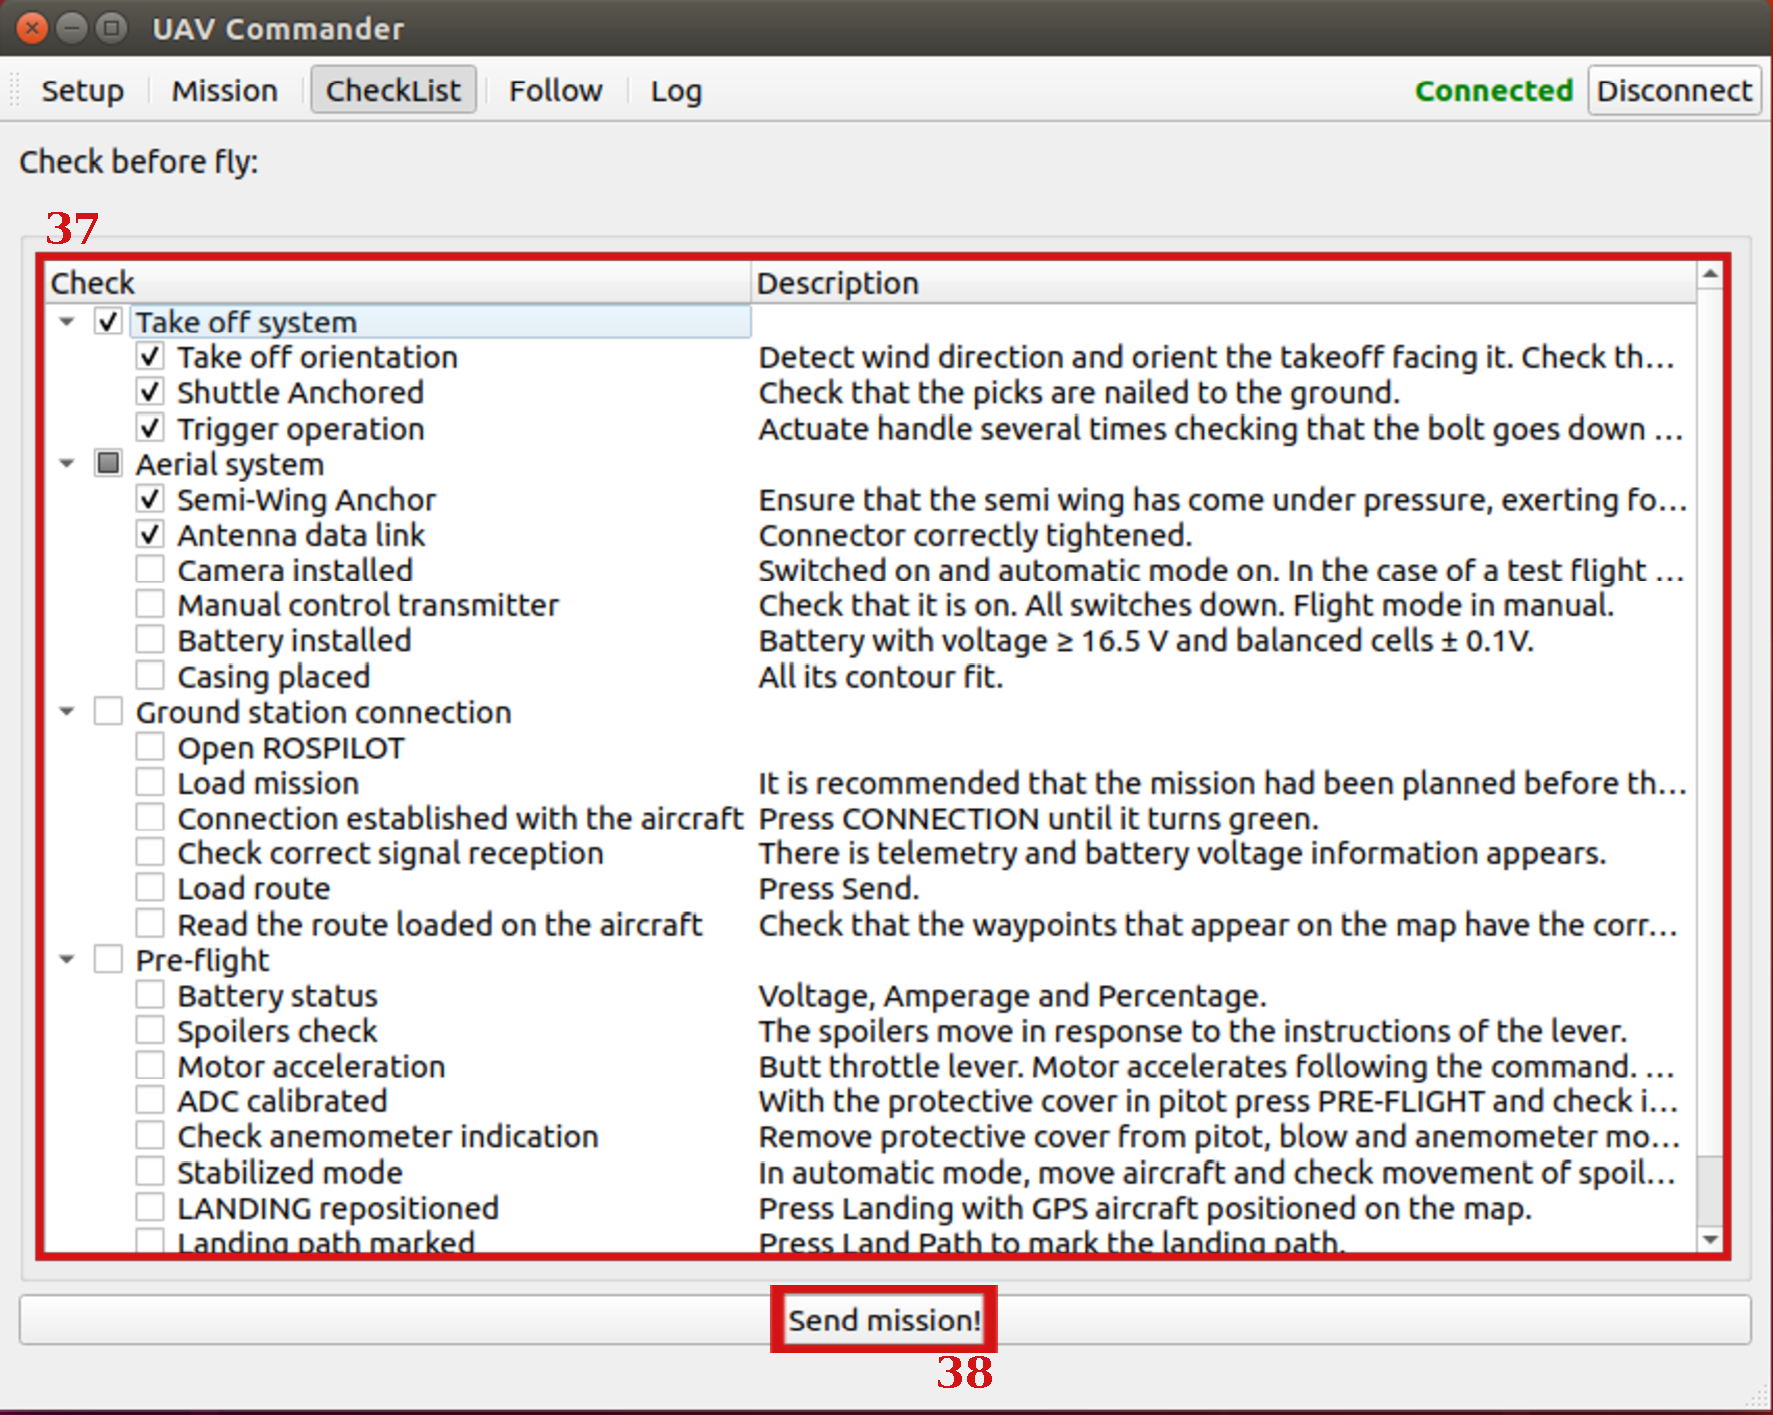
\includegraphics[width=\textwidth]{figures/man/checklist.pdf}
\end{figure}

\begin{table}[H]
    \centering
    \begin{threeparttable}
        \begin{tabular}{| l | l |}
            \hline
            \thead{Nº} & \thead{Descripción} \\ \hline
            
            37 & Listado de comprobaciones pre-vuelo. \\ \hline
            38 & Botón para enviar la misión a la aeronave. \\ \hline
        \end{tabular}
        
    \end{threeparttable}
\end{table}

\clearpage

\subsubsection{Pestaña \emph{Follow}} \label{subsubsection:man-follow}
La pestaña \emph{Follow} permite el seguimiento en tiempo real de la aeronave. El seguimiento se realiza a través de la posición gracias a la escena y a través de los datos de navegación gracias a la ventana secundaria de sensores (Secc. \ref{subsubsection:man-sensor}).

\begin{figure}[H]
    \centering
    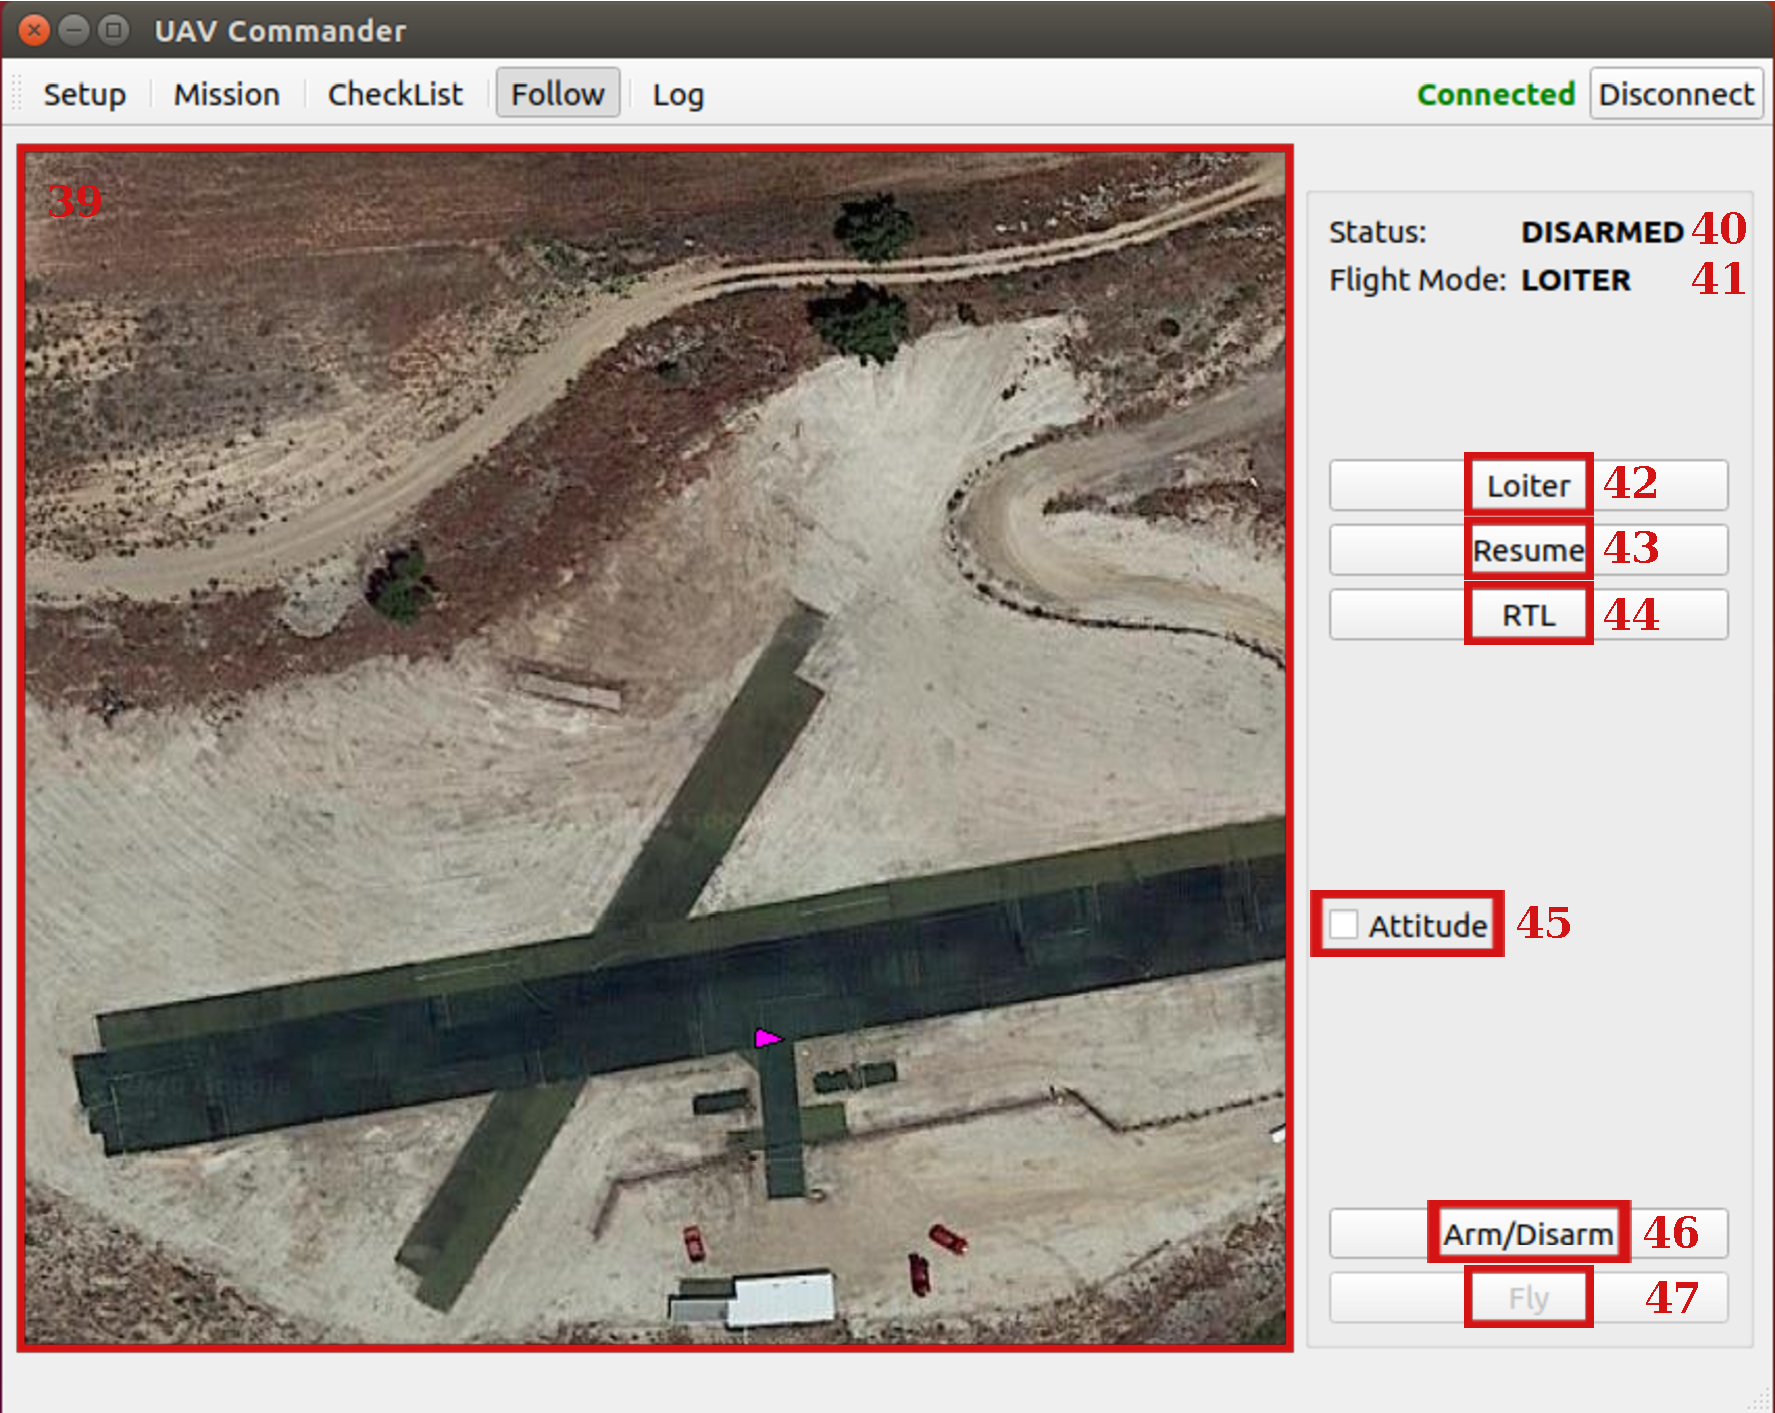
\includegraphics[width=\textwidth]{man/follow.pdf}
\end{figure}

\begin{table}[H]
    \centering
    \begin{threeparttable}
        \begin{tabular}{| l | l |}
            \hline
            \thead{Nº} & \thead{Descripción} \\ \hline
            
            39 & Escena con el mapa cargado. \\ \hline
            40 & Etiqueta que muestra el estado de la aeronave. \\ \hline
            41 & Etiqueta que muestra el modo de vuelo de la aeronave. \\ \hline
            42 & Botón para activar el modo de vuelo \emph{Loiter}. \\ \hline
            43 & Botón para activar el modo de vuelo \emph{Auto}. \\ \hline
            44 & Botón para activar el modo de vuelo \emph{RTL}. \\ \hline
            45 & Botón para abrir la pestaña secundaria de sensores (Ver \ref{subsubsection:man-sensor}). \\ \hline
            46 & Botón para armar/desarmar. \\ \hline
            47 & Botón para despegar e iniciar misión. \\ \hline
        \end{tabular}
        
    \end{threeparttable}
\end{table}

\clearpage

\subsubsection{Pestaña \emph{Log}} \label{subsubsection:man-log}
La pestaña \emph{Log} permite la obtención de datos post-vuelo de la aeronave.

\begin{figure}[H]
    \centering
    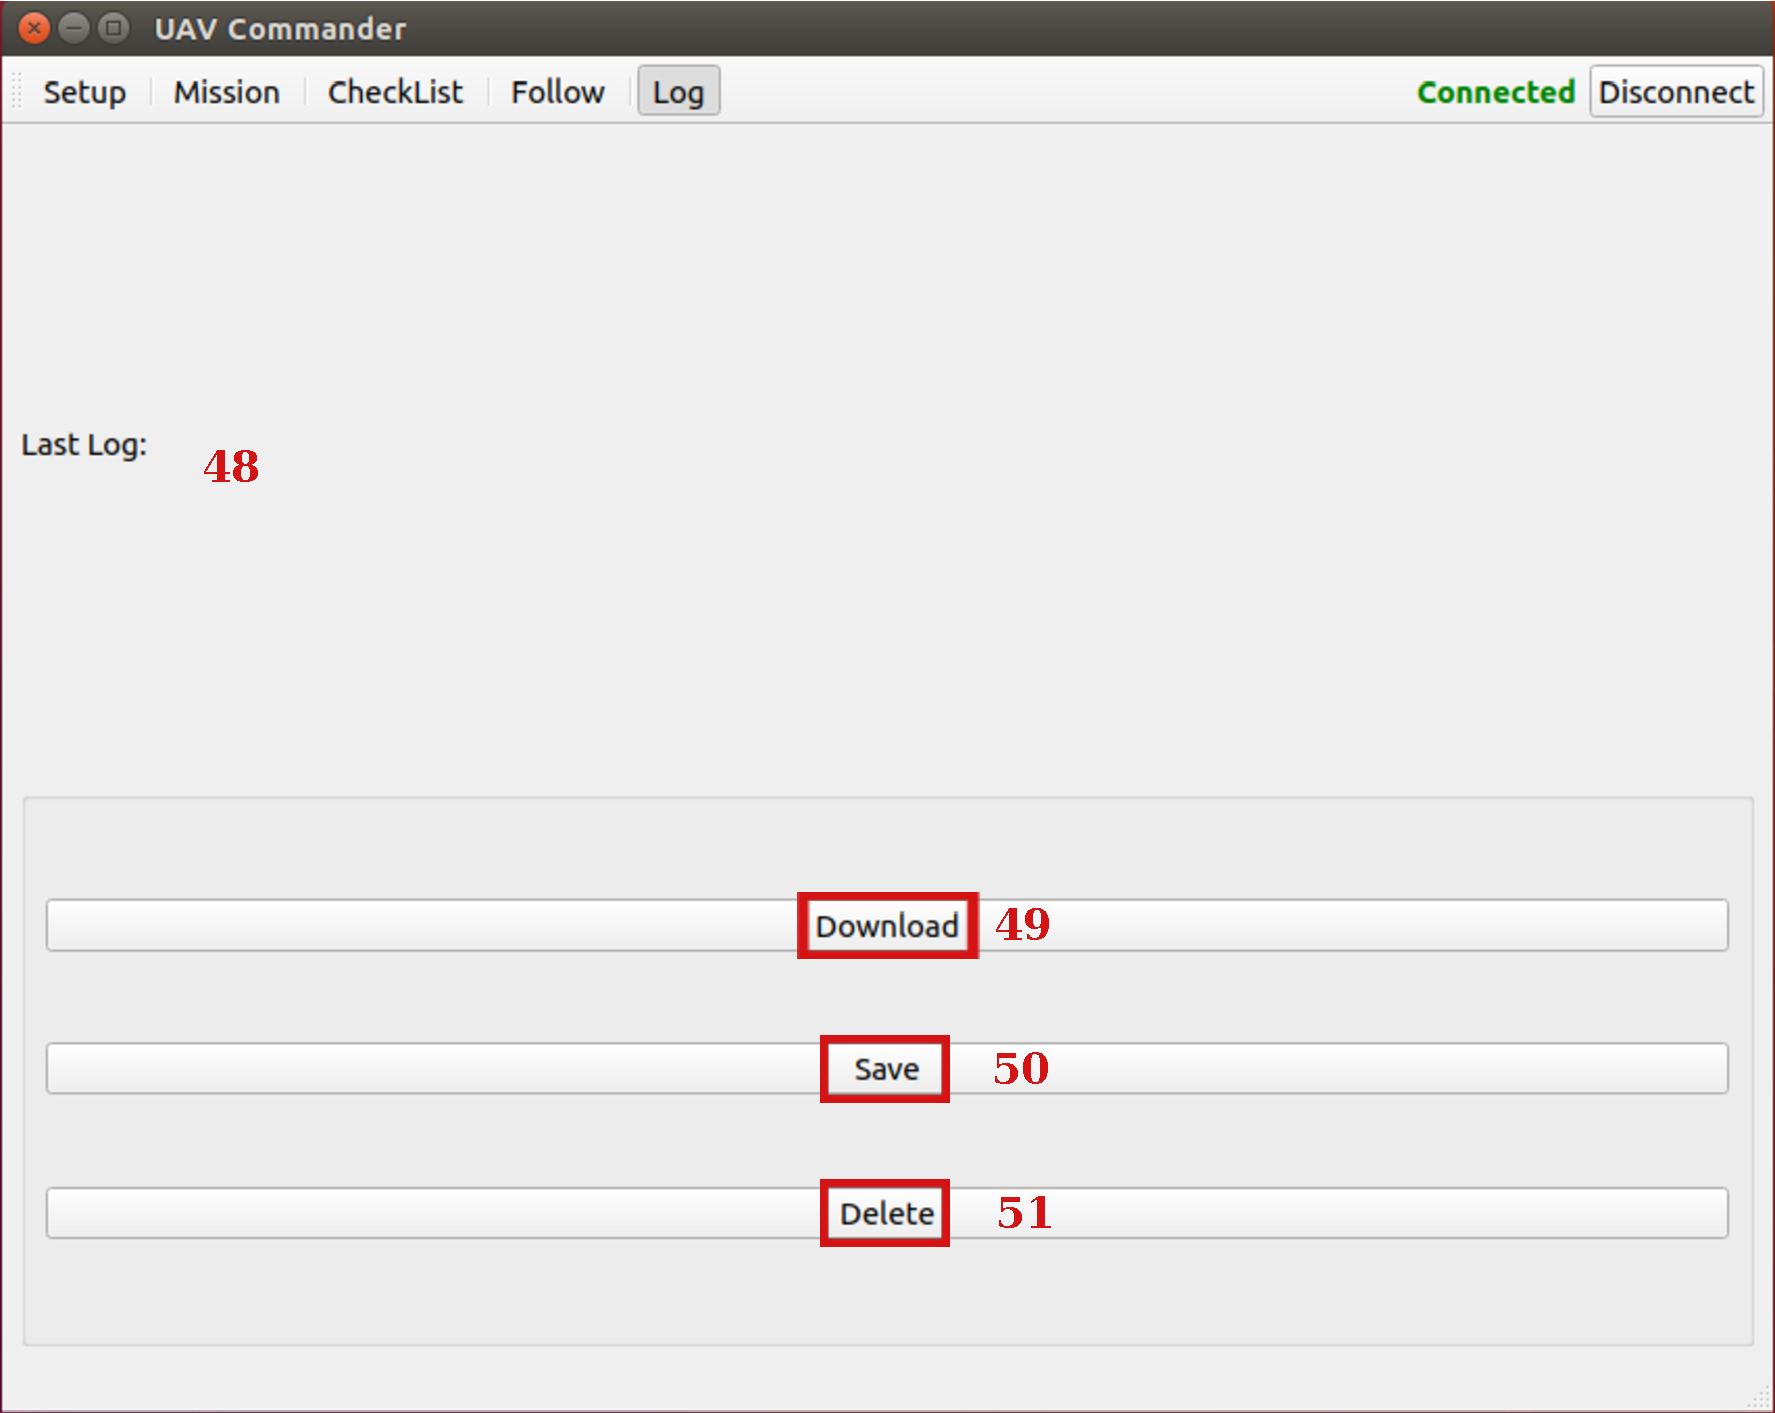
\includegraphics[width=\textwidth]{man/log.pdf}
\end{figure}

\begin{table}[H]
    \centering
    \begin{threeparttable}
        \begin{tabular}{| l | l |}
            \hline
            \thead{Nº} & \thead{Descripción} \\ \hline
            
            48 & Etiqueta que muestra último log descargado. \\ \hline
            49 & Botón para descargar los logs del autopiloto. \\ \hline
            50 & Botón para guardar los logs descargados. \\ \hline
            51 & Botón para borrar los logs del autopiloto. \\ \hline
        \end{tabular}
        
    \end{threeparttable}
\end{table}

\clearpage

\subsection{Ventanas Secundarias} \label{subsection:man-vent-sec}
La ventanas secundarias son desplegadas a través del menú o de la ventana principal y complementan las acciones de la aplicación. Entre las ventanas secundarias disponibles se encuentran la ventana de configuración (Secc. \ref{subsubsection:man-config}), la ventana de carga de mapas locales (Secc. \ref{subsubsection:man-local}), la ventana de puntos de paso (Secc. \ref{subsubsection:man-puntos}) y la ventana de sensores (Secc. \ref{subsubsection:man-sensor}).

\subsubsection{Ventana de Configuración} \label{subsubsection:man-config}
La ventana de configuración permite modificar parámetros de la escena y el idioma de la aplicación de forma dinámica.

\begin{figure}[H]
    \centering
    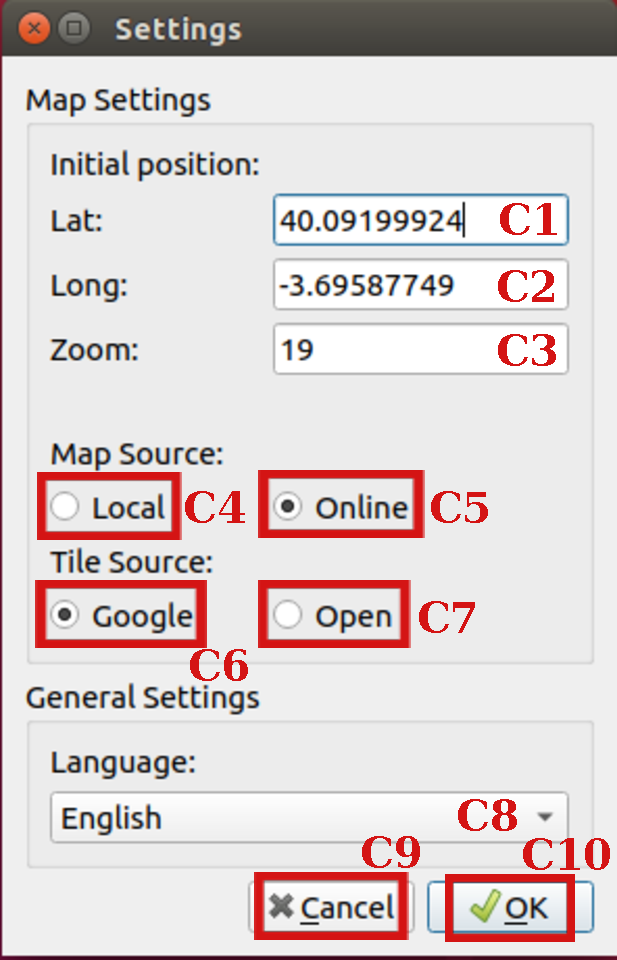
\includegraphics[width=0.4\textwidth]{man/settings.pdf}
\end{figure}

\begin{table}[H]
    \centering
    \begin{threeparttable}
        \begin{tabular}{| l | l |}
            \hline
            \thead{Nº} & \thead{Descripción} \\ \hline
            
            C1  & Latitud por defecto de la escena (º). \\ \hline
            C2  & Longitud por defecto de la escena (º). \\ \hline
            C3  & Zoom por defecto de la escena. \\ \hline
            C4  & Botón para activar mapas locales sobre la escena. \\ \hline
            C5  & Botón para activar mapas en línea sobre la escena. \\ \hline
            C6  & Botón para activar mapas de Google sobre la escena. \\ \hline
            C7  & Botón para activar mapas abiertos sobre la escena. \\ \hline
            C8  & Desplegable para seleccionar el idioma de la interfaz gráfica de usuario. \\ \hline
            C9  & Botón para cancelar cambios. \\ \hline
            C10 & Botón para confirmar cambios. \\ \hline
        \end{tabular}
        
    \end{threeparttable}
\end{table}

\clearpage

\subsubsection{Ventana de carga de Mapa Local} \label{subsubsection:man-local}
La ventana de carga de mapas locales permite abrir ficheros locales con datos ortofotográficos y desplegarlos sobre la escena. 

\begin{figure}[H]
    \centering
    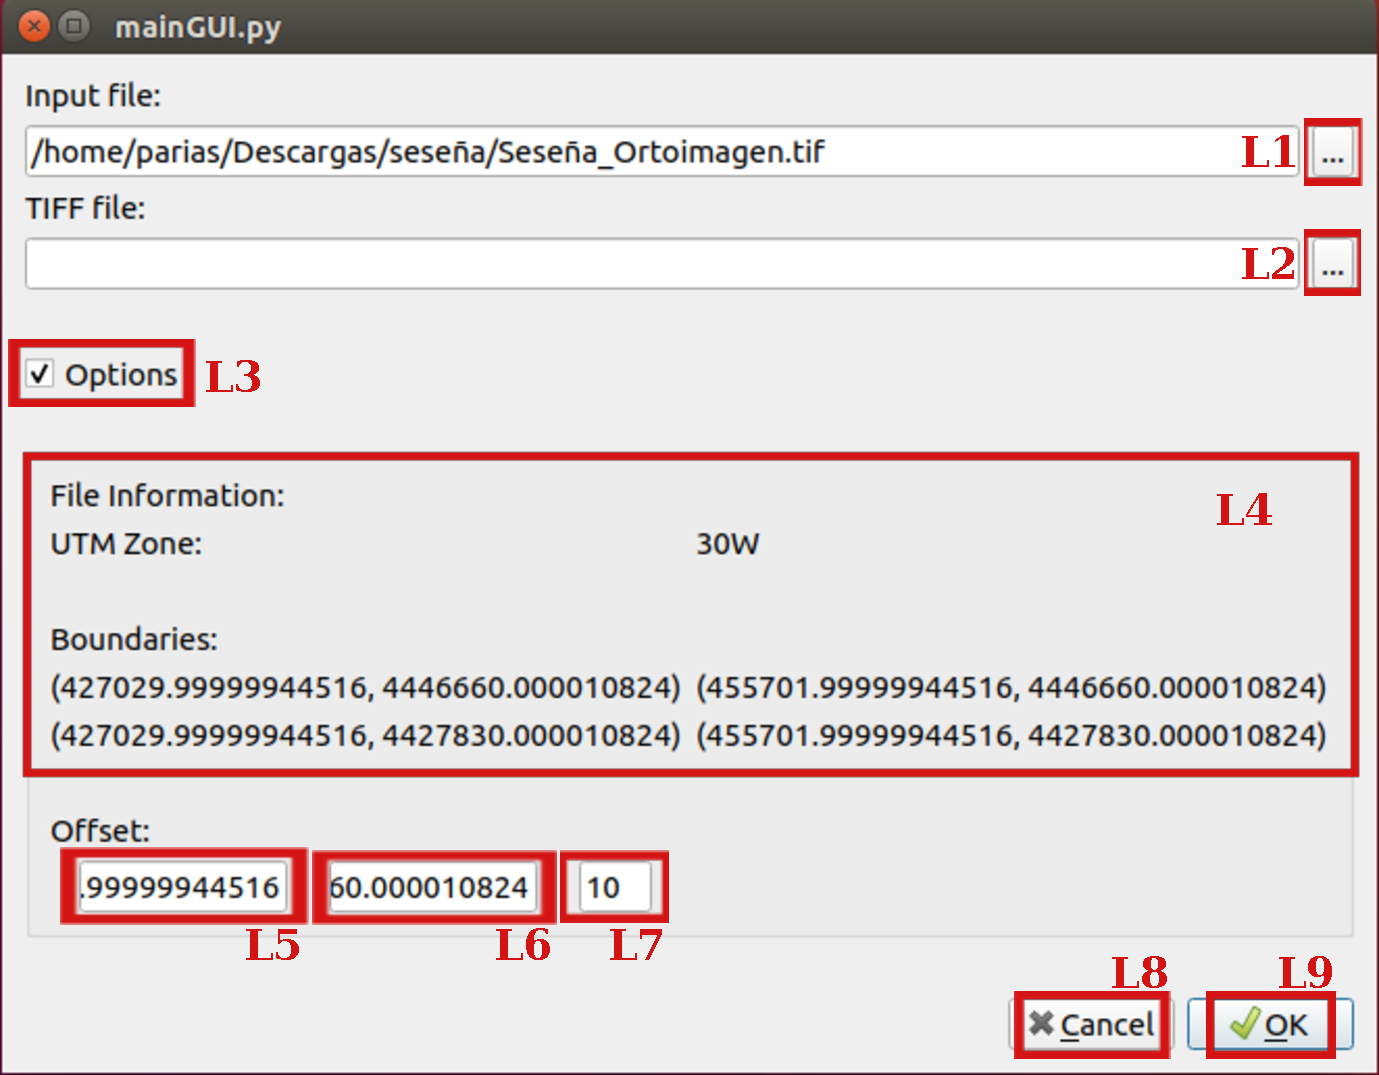
\includegraphics[width=0.8\textwidth]{man/local_map.pdf}
\end{figure}

\begin{table}[H]
    \centering
    \begin{threeparttable}
        \begin{tabular}{| l | l |}
            \hline
            \thead{Nº} & \thead{Descripción} \\ \hline
            
            L1 & Botón para cargar archivo con ortoimagen. \\ \hline
            L2 & Botón para cargar archivo con elevaciones. \\ \hline
            L3 & Botón para ostrar/ocultar opciones. \\ \hline
            L4 & Información sobre ortoimagen cargada. \\ \hline
            L5 & Coordenada X (UTM) a cargar (m). \\ \hline
            L6 & Coordenada Y (UTM) a cargar (m). \\ \hline
            L7 & Zoom a cargar. \\ \hline
            L8 & Botón para cancelar cambios. \\ \hline
            L9 & Botón para confirmar cambios. \\ \hline
        \end{tabular}
        
    \end{threeparttable}
\end{table}

\clearpage

\subsubsection{Ventana de Puntos de Paso} \label{subsubsection:man-puntos}
La ventana de puntos de paso permite desplegar una lista con los puntos de paso que componen una misión.

\begin{figure}[H]
    \centering
    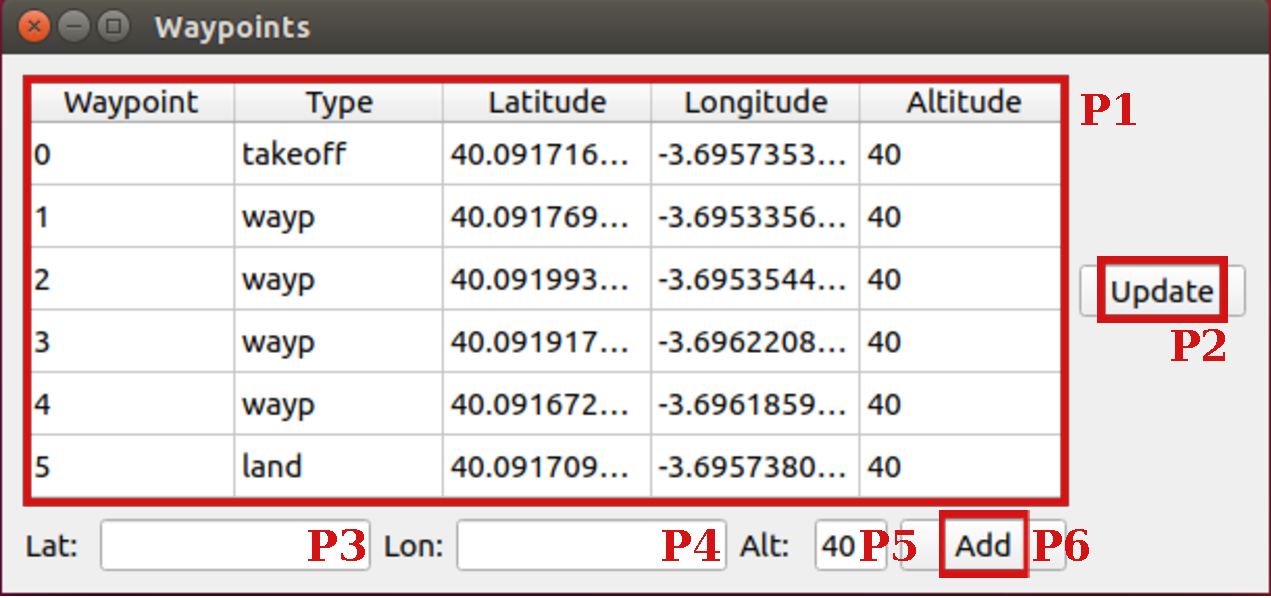
\includegraphics[width=0.8\textwidth]{man/wayp_window.pdf}
\end{figure}

\begin{table}[H]
    \centering
    \begin{threeparttable}
        \begin{tabular}{| l | l |}
            \hline
            \thead{Nº} & \thead{Descripción} \\ \hline
            
            P1 & Lista con los puntos de paso de la misión. \\ \hline
            P2 & Botón para actualizar los puntos de la lista sobre la escena. \\ \hline
            P3 & Latitud (º). \\ \hline
            P4 & Longitud (º). \\ \hline
            P5 & Altura (m). \\ \hline
            P6 & Botón para añadir un punto de paso a la lista. \\ \hline
        \end{tabular}
        
    \end{threeparttable}
\end{table}

\clearpage

\subsubsection{Ventana de Sensores} \label{subsubsection:man-sensor}
La ventana de sensores muestra los datos de navegación de la aeronave a través de útiles de aeronavegación estándar.

\begin{figure}[H]
    \centering
    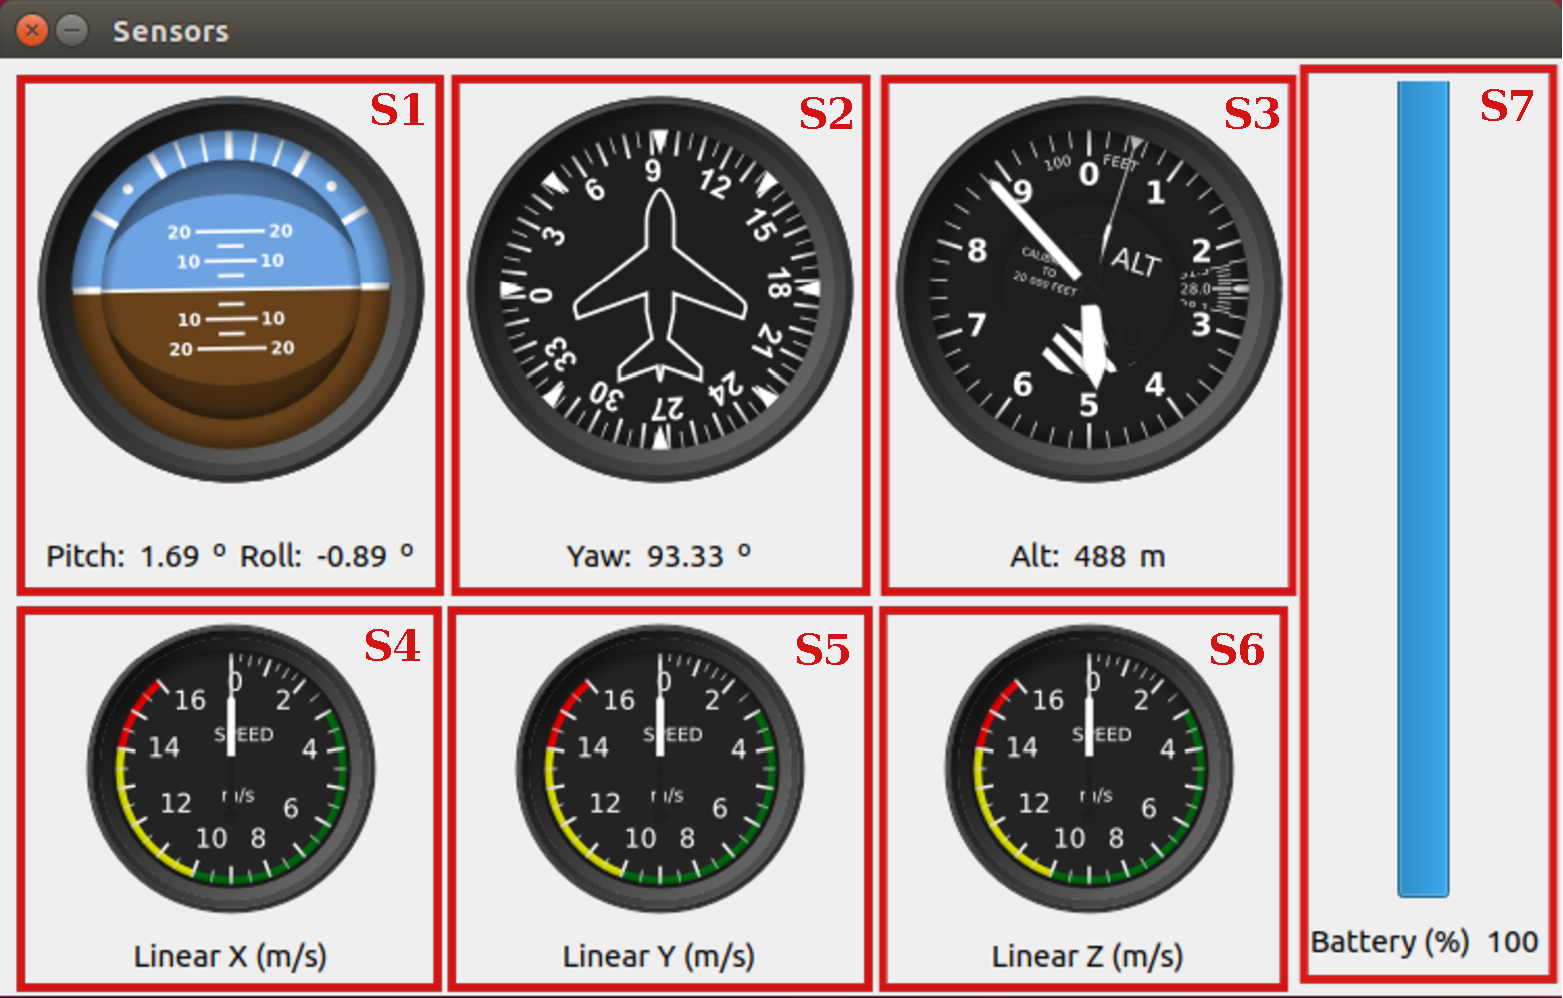
\includegraphics[width=\textwidth]{man/sensors.pdf}
\end{figure}

\begin{table}[H]
    \centering
    \begin{threeparttable}
        \begin{tabular}{| l | l |}
            \hline
            \thead{Nº} & \thead{Descripción} \\ \hline
            
            S1 & Horizonte artificial. \\ \hline
            S2 & Indicador de rumbo. \\ \hline
            S3 & Altímetro. \\ \hline
            S4 & Velocidad lineal X. \\ \hline
            S5 & Velocidad lineal Y. \\ \hline
            S6 & Velocidad lineal Z. \\ \hline
            S7 & Batería. \\ \hline
        \end{tabular}
        
    \end{threeparttable}
\end{table}

\clearpage

\section{Casos de uso}
Las diferentes pruebas se reúnen en los diferentes casos de uso, a los cual se les dedica una de las subsecciones de esta sección. Los casos de uso expuestos en este capítulo son ocho:

\begin{enumerate}
    \item Caracterización de una aeronave y su carga de pago.
    \item Carga de un mapa local en una determinada posición.
    \item Creación y posterior guardado en fichero de una misión polilínea.
    \item Establecimiento de conexión con la aeronave.
    \item Creación de una misión por patrón y validación de la misma.
    \item Carga de una misión en fichero, envío y seguimiento de la misión.
    \item Interrupción de una misión y vuelta a casa.
    \item Cambio de idioma de la aplicación.
\end{enumerate}

Además, el Apéndice \ref{chapter:use-case} recoge una tabla que esquematiza cada uno de los casos de uso. Junto a las tablas se añaden una serie de diagramas de caso de uso que tratan de ejemplificar la interacción entre el usuario y la aplicación para cada caso. \\

\subsection{Caso de uso 1: Caracterización de una aeronave y su carga de pago.} \label{subsection:results-caso1}
El primer caso de uso describe una situación en la que un operario cualquiera desee caracterizar una aeronave y su carga de pago mediante la introducción de sus parámetros en la aplicación. La tabla con el caso de uso se presenta en el Apéndice \ref{section:app-caso1}. \\
Para poder realizar la acción requerida, la aplicación debe estar abierta y en ejecución. Los diferentes pasos de una secuencia normal serían:

\begin{enumerate}
    \item En primer lugar, hay que pinchar sobre \emph{Setup} para desplegar dicha pestaña.
    \item A continuación, el usuario debe completar los diferentes campos requeridos sobre la configuración de la aeronave. Todo aquel parámetro que permanezca en blanco tomará un valor nulo.
    \item El operario, tras comprobar los datos introducidos, pincha sobre el botón \emph{Submit} para caracterizar la aeronave y su carga de pago.
    \item En caso de cometer algún error al introducir los datos o de querer modificar algún parámetro, se podrían modificar los campos necesarios y confirmar estos cambios pinchando sobre el botón \emph{Submit}.
    \item Para guardar una configuración creada para un uso futuro de la misma, es necesario pinchar sobre el botón \emph{Save} para generar un archivo de configuración. Sobre la ventana emergente hay que elegir un nombre y una ubicación de guardado, y posteriormente pinchar en el botón \emph{Save}.
\end{enumerate}

En el paso dos, si el operario hubiese creado un fichero de configuración anteriormente, podría cargarlo directamente en la aplicación, evitando repetir el proceso. Para ello se debe pinchar en el botón \emph{Load} y seleccionar el archivo de configuración a cargar. Tras seleccionar el archivo es necesario pinchar en el botón \emph{Open} sobre la ventana emergente. \\
Es importante destacar que no es posible tener más de un archivo de configuración abierto al mismo tiempo. Además, en caso de tener un fichero de configuración abierto, cualquier cambio realizado sobre el mismo debe ser confirmado pinchando sobre el botón \emph{Submit} para que tenga efecto sobre el modelo de configuración. Por otro lado, si estos cambios quieren ser guardados de forma persistente sobre el archivo de configuración, es necesario pinchar sobre el botón \emph{Save}. Esta acción sobrescribirá el archivo abierto y no creará un archivo de configuración nuevo.


\subsection{Caso de uso 2: Carga de un mapa local en una determinada posición.} \label{subsection:results-caso2}
En este caso de uso se explica el proceso de carga de un mapa local mostrando una posición determinada en la aplicación. En el Apéndice \ref{section:app-caso2} se muestra una tabla que recoge el caso de uso. \\
Este ejemplo requiere que la aplicación se encuentre abierta y en ejecución. Además, es necesario disponer de un archivo de imagen geo-referenciada con la ubicación precisada. Estos archivos pueden ser obtenido desde la página web del Instituto Geográfico Nacional \cite{ign}. Solo dos formatos son admitidos, las extensiones TIFF y ECW. \\
Una secuencia normal ejecutada por un usuario cualquiera sería:

\begin{enumerate}
    \item Para comenzar, el operario debe pinchar sobre \emph{Mission} para abrir la pestaña con el mismo nombre.
    \item Con el objetivo de abrir la ventana secundaria de carga de mapas locales, hay que pinchar sobre el botón \emph{Local Map}.
    \item Pinchando sobre el primer botón \emph{...} del campo \emph{Input File} se abriría una ventana de carga sobre la que se debe buscar y seleccionar el archivo con el mapa local. A continuación, confirmar el archivo pinchando sobre el botón \emph{Open}.
    \item Existe la posibilidad de cargar también un archivo con información acerca de la altitud del terreno. Ambos archivos deben coincidir en la ubicación comprendida en sus datos. Pinchando sobre el segundo botón \emph{...} del campo \emph{TIFF File} se abriría otra ventana de carga. Al igual que en el paso anterior, se debe buscar el archivo de elevaciones, seleccionarlo y pinchar sobre el botón \emph{Open} para cargar el fichero.
    \item Para modificar la posición inicial desplegada en la escena, hay que pinchar sobre la opción \emph{Options}. Esto muestra la información asociada al mapa local. Modificando los campos \emph{Offset} se puede modificar la posición inicial cargada, que por defecto muestra la esquina superior izquierda de la imagen. 
    \item Finalmente, para confirmar la acción, el usuario debe pinchar sobre el botón \emph{OK} y en la escena se podría observar el mapa cargado.
\end{enumerate}

En caso de que la posición inicial introducida no fuese válida por encontrarse fuera de la superficie abarcada por el fichero, la aplicación no mostraría ningún error al usuario. Sin embargo, la escena no mostraría ninguna imagen y permanecería mostrando una imagen en blanco, pues sobre esa posición no dispone de información a mostrar. Para modificar la posición mostrada en la escena, se recomienda repetir el caso de uso.

\subsection{Caso de uso 3: Creación y posterior guardado en fichero de una misión polilínea.} \label{subsection:results-caso3}
Este caso de uso prueba las acciones necesarias para la creación y posterior guardado de una misión polilínea. El Apéndice \ref{section:app-caso3} recoge el caso de uso simplificado en una tabla. \\
El único requisito para poder completar este experimento radica en tener abierta y en ejecución la aplicación. La secuencia normal de ejecución se resume en los siguientes puntos:

\begin{enumerate}
    \item Primeramente, la aplicación debe mostrar la pestaña \emph{Mission}. Para ello, hay pinchar en \emph{Mission} sobre el menú de la ventana principal.
    \item Si la escena no mostrase la ubicación sobre la que se quiere crear la misión, la posición se podría modificar introduciendo la latitud y longitud sobre los campos \emph{Lat} y \emph{Long} y pinchando sobre el botón \emph{Search}.
    \item Tras obtener el mapa deseado, el usuario debe pinchar sobre el botón \emph{Waypoint} para abrir el creador de misiones por polilínea. 
    \item A la hora de crear la misión, es necesario introducir el punto de despegue en primer lugar. Para ello hay que pinchar sobre el botón \emph{Take Off} y después pinchar sobre el mapa en el punto deseado de despegue. La altura introducida en el campo \emph{Height} es la altura necesaria a alcanzar antes de comenzar la misión.
    \item A continuación se añadirán los puntos de paso deseados por el usuario. Para añadir un punto de paso se debe pinchar sobre el mapa en la posición querida y con la altura asociada al campo \emph{Height}.
    \item Para crear el punto de aterrizaje, el usuario pinchará sobre el botón \emph{Land} y posteriormente pinchará sobre el mapa la posición deseada de aterrizaje.
    \item Finalmente, para guardar la misión, el usuario debe pinchar sobre el botón \emph{Save} con la misión ya creada completamente. Una ventana de guardado emergerá donde se debe seleccionar un nombre y una ubicación de guardado para el nuevo fichero de misión. Para confirmar el guardado, se debe pinchar sobre el botón \emph{Save} de esta ventana.
\end{enumerate}

El mapa utilizado puede ser cualquiera de los soportados por la aplicación. Si se desea utilizar un mapa local, este se puede cargar siguiendo el caso de uso 2 (Secc. \ref{subsection:results-caso2}). Sin embargo, si el usuario no dispusiese de una archivo de mapa local ni tampoco de conexión a internet y los mapas no estuvieran previamente cacheados, no se podría obtener un mapa válido sobre el que crear la misión. Por ello, la acción no sería realizable y habría que posponerla a una situación en la que se dispusiese de algún mapa. \\
Por otro lado, los puntos se pueden introducir también mediante los campos de latitud, longitud y altura que lo posicionan en el espacio. Tanto el punto de despegue, el punto de aterrizaje o los puntos de paso se pueden añadir de esta forma alternativa. Para ello es necesario abrir la ventana secundaria con la lista de los puntos en la misión. Esta ventana se puede abrir pinchando en el botón \emph{Add Waypoint} en el menú de creador de misiones. Sobre la ventana se encuentran los campos \emph{Lat}, \emph{Lon} y \emph{Alt} junto al botón \emph{Add} con los que se pueden añadir puntos a la misión. \\
Si el usuario cometiese un error introduciendo alguno de los puntos de la misión, sería necesario pinchar el botón \emph{Clear} para borrar la misión y empezar de nuevo la creación de la misma. \\
Es importante destacar que no es posible crear más de una misión al mismo tiempo. En caso de tener un archivo de misión abierto, cualquier cambio sobre la misma sobrescribirá el archivo al guardar los cambios (pinchando en el botón \emph{Save}) y no creará un archivo de misión nuevo. \\

\subsection{Caso de uso 4: Establecimiento de conexión con la aeronave.} \label{subsection:results-caso4}
El cuarto caso de uso explica el procedimiento a seguir para establecer la conexión entre la aeronave y la estación de tierra. Se agrega en el Apéndice \ref{section:app-caso4} una tabla resumen y simplificada de lo que en esta sección se describe. \\
Para una perfecta ejecución del caso de uso es necesario que la aplicación se encuentre abierta y en ejecución. A su vez, la aeronave debe estar encendida y con el posicionamiento GPS establecido. La siguiente secuencia recoge los pasos a seguir en situaciones normales:

\begin{enumerate}
    \item Para tratar de establecer la conexión hay que pinchar sobre el botón \emph{Connect} situado en el menú de la ventana principal.
    \item En caso de un establecimiento de conexión favorable, la etiqueta de estado de conexión en el menú cambiará a color verde mostrando el texto \emph{Connected}.
\end{enumerate}

Es importante resaltar que si la conexión no se puede establecer debido a algún error, la aplicación debe ser reiniciada para poder volver a realizar un intento de establecimiento de conexión. También hay que tener en cuenta que el establecimiento puede durar unos segundos en función del estado de la aeronave.

\subsection{Caso de uso 5: Creación de una misión por patrón y validación de la misión.} \label{subsection:results-caso5}
El quinto caso de uso muestra como deberá comportarse la aplicación frente a la intención por parte de un usuario para crear una misión y la validación de la misma. Esta acción conlleva los requisitos de que la aplicación se encuentre abierta y en ejecución, y de que la aeronave se encuentre caracterizada. Para una correcta configuración de la aeronave se puede seguir el caso de uso 1 (Secc. \ref{subsection:results-caso1}).
Con caso de uso se presenta también una tabla en el Apéndice \ref{section:app-caso5} que recoge sus principales aspectos. La secuencia normal de ejecución es la siguiente:

\begin{enumerate}
    \item La pestaña \emph{Mission} debe estar activa. Para ello hay que pinchar en el menú con si mismo nombre \emph{Mission}.
    \item Si la escena no mostrase la ubicación sobre la que se quiere crear la misión, la posición se podría modificar introduciendo la latitud y longitud sobre los campos \emph{Lat} y \emph{Long} y pinchando sobre el botón \emph{Search}.
    \item Tras obtener el mapa deseado, el usuario debe pinchar sobre el botón \emph{Pattern} para abrir el creador de misiones por patrón.
    \item Para fijar la altura de vuelo durante la ruta de escaneo, se debe modificar el valor del campo \emph{Height}.
    \item A continuación se añadirán los vértices del polígono a escanear. Se podrán añadir tantos vértices como el usuario desee con un mínimo de tres vértices. Para añadir cada vértice, el operario debe pinchar sobre el mapa en la posición donde desee añadir cada vértice.
    \item Para finalizar y cerrar el polígono se debe pinchar sobre el botón \emph{Close Pattern}. Este paso genera la ruta de escaneo y la misión se mostrará sobre la escena.
    \item El usuario puede guardar la misión creada para un uso futuro pinchando sobre el botón \emph{Save}. Sobre la ventana emergente se debe elegir el nombre y la ubicación de guardado para el archivo de misión y pinchar sobre el botón \emph{Save} para confirmar el guardado.
    \item Finalmente, para validar la misión hay que pinchar sobre el botón \emph{Submit}. Una ventana mostrará un aviso conforme la misión ha sido aceptada o rechazada.
\end{enumerate}

El mapa utilizado puede ser cualquiera de los soportados por la aplicación. Si se desea utilizar un mapa local, este se puede cargar siguiendo el caso de uso 2 (Secc. \ref{subsection:results-caso2}). Sin embargo, si el usuario no dispusiese de una archivo de mapa local ni tampoco de conexión a internet y los mapas no estuvieran previamente cacheados, no se podría obtener un mapa válido sobre el que crear la misión. Por ello, la acción no sería realizable y habría que posponerla a una situación en la que se dispusiese de algún mapa. \\
Por otro lado, los vértices se pueden introducir también mediante los campos de latitud y longitud. Para ello es necesario abrir la ventana secundaria con la lista de los vértices del polígono. Esta ventana se puede abrir pinchando en el botón \emph{Add Pattern} en el menú de creador de misiones por patrón. Sobre la ventana se encuentran los campos \emph{Lat} y \emph{Lon} junto al botón \emph{Add} con los que se pueden añadir los vértices al polígono. \\
Si el usuario cometiese un error introduciendo alguno de los vértices del polígono, sería necesario pinchar el botón \emph{Clear} para borrar el polígono y empezar de nuevo la creación del mismo. \\
Finalmente, la ruta de escaneo solo se puede crear si la aeronave ha sido correctamente caracterizada. Por ello, si la aeronave no ha sido configurada en la aplicación, durante el paso 6 saldrá un mensaje de error avisando al usuario que debe caracterizar a la aeronave antes de cerrar el polígono y crear la misión por patrón. La aeronave se puede caracterizar siguiendo el caso de uso 1 (Secc. \ref{subsection:results-caso1}) y a continuación, se puede continuar este caso de uso desde el paso 6. \\

Es importante destacar que al igual que sucedía con las misiones polilínea, no es posible crear más de una misión al mismo tiempo. Además, en caso de tener un archivo de misión abierto, cualquier cambio que se grabe de forma persistente pinchando sobre el botón \emph{Save} sobrescribirá al archivo abierto y no creará un archivo de misión nuevo.

\subsection{Caso de uso 6: Carga de una misión en fichero, envío y seguimiento de la misión.} \label{subsection:results-caso6}
Este caso de uso describe la carga de una misión en fichero a la aplicación, la validación y el envío de la misión, seguido de un posterior seguimiento de la misión. Son varios los requisitos asociados a este caso de uso. En primer lugar, la aplicación debe estar abierta y en ejecución. En segundo lugar, la conexión a la aeronave debe haber sido correctamente establecida siguiendo el caso de uso 4 (Secc. \ref{subsection:results-caso4}). Además, una misión debe haber sido creada y guardada en un fichero previamente. Los casos de usos 3 y 5 muestran como crear los distintos tipos de misión (Secc. \ref{subsection:results-caso3} y \ref{subsection:results-caso5}). \\
En el Apéndice \ref{section:app-caso6} se presenta este caso de uso en formato de tabla con los principales aspecto esquematizados. La secuencia normal de ejecución es la siguiente:

\begin{enumerate}
    \item En primer lugar, se debe pinchar sobre \emph{Mission} para desplegar dicha pestaña.
    \item A continuación, para cargar una misión es necesario pinchar sobre el botón \emph{Load}. Sobre la ventana emergente, el operario selecciona el archivo de misión deseado y pincha sobre el botón \emph{Open} para confirmar la selección.
    \item Para validar la misión se pincha sobre el botón \emph{Submit}. Un aviso mostrará al usuario si la misión ha sido aceptada o rechazada. Si la misión es válida, la aplicación pasará a mostrar la pestaña \emph{Checklist}.
    \item Sobre la nueva pestaña se debe completar y validar cada caja de validación. Cada elemento corresponde a una medida de seguridad que se debe comprobar antes de un vuelo. Tras completar cada una de las comprobaciones, el usuario podrá pinchar sobre el botón \emph{Send Mission} para el envío de la misión a la aeronave. Al pinchar sobre el botón se mostrará la pestaña \emph{Follow}.
    \item Para iniciar la misión es necesario armar la aeronave pinchando sobre el botón \emph{Arm} y a continuación pinchar sobre el botón \emph{Fly} para despegar.
    \item Durante el seguimiento de vuelo el operario podrá observar los parámetros de vuelo pinchando sobre la opción \emph{Attitude} que desplegará una ventana secundaria con los útiles de navegación.
\end{enumerate}

A la hora de cargar la misión en la aplicación, si esta es una misión de patrón, la aeronave debe haber sido previamente caracterizada, de lo contrario no se podrá cargar la misión. Para caracterizar la aeronave correctamente se recomienda seguir el caso de uso 1 (Secc. \ref{subsection:results-caso1}). \\
Si durante el paso 3 la misión no ha sido aceptada, el usuario deberá crear o cargar otra misión válida. Los casos de uso 3 y 5 muestran la creación de misiones válidas (Secc. \ref{subsection:results-caso3} y \ref{subsection:results-caso5}). \\
Finalmente, para poder enviar la misión a la aeronave la conexión tiene que haber sido establecida previamente. Si la conexión no ha sido establecida, un error se mostrará durante el paso 4. Para establecer la conexión se recomienda seguir el caso de uso 4 (Secc. \ref{subsection:results-caso4}).\\

\subsection{Caso de uso 7: Interrupción de una misión y vuelta a casa.} \label{subsection:results-caso7}
Este caso de uso recoge los pasos necesarios para la interrupción de una misión y la vuelta a casa de la aeronave. Para que esta situación tenga lugar, la aplicación debe estar abierta, en ejecución, con conexión establecida y con una misión en curso. En el cuarto caso de uso (Secc. \ref{subsection:results-caso4}) se explica el procedimiento para establecer la conexión, mientras que en el sexto caso de uso (Secc. \ref{subsection:results-caso6}) se recogen los pasos para el inicio y el seguimiento de una misión en modo automático. \\
Este caso de uso se presenta en formato de tabla en el Apéndice \ref{section:app-caso7}. La secuencia de ejecución en condiciones normales es la siguiente:

\begin{enumerate}
    \item La pestaña \emph{Follow} debe estar activa. Para ello es necesario pinchar en el menú con el mismo nombre en la ventana principal. En esta pestaña se pueden observar las actuaciones de la aeronave en todo momento.
    \item Para iniciar la vuelta a casa, el operario debe pinchar sobre el botón \emph{RTL}. Tras esto, la aeronave cambiará su modo de vuelo a \emph{RTL} e iniciará la ruta de retorno.
\end{enumerate}

El usuario puede decidir anular el retorno a casa. Para ello dispone de dos modos de vuelo. En primer lugar, pinchando sobre el botón \emph{Loiter} se activaría el modo de vuelo \emph{Hold} o \emph{Loiter}, donde la aeronave mantendría la posición en el momento de activación. En segundo lugar, pinchando sobre el botón \emph{Resume}, la aeronave volvería al modo de vuelo automático y continuaría con la misión interrumpida.

\subsection{Caso de uso 8: Cambio de idioma de la aplicación.} \label{subsection:results-caso8}
Finalmente, el último caso de uso presentado muestra como cambiar dinámicamente el idioma del texto de la aplicación. La aplicación debe estar abierta y en ejecución. El Apéndice \ref{section:app-caso8} incluye una tabla con el caso de uso esquematizado. La secuencia de ejecución en condiciones normales es la siguiente:

\begin{enumerate}
    \item En primer lugar, es necesario acceder a la ventana secundaria de ejecución siguiendo la ruta \emph{File - Settings - More Settings} en el menu de fichero de la aplicación.
    \item Sobre la ventana de configuración desplegada se debe elegir en la lista desplegabe \emph{Language} uno de los idiomas disponibles. Para confirmar los cambios hay que pinchar sobre el botón \emph{OK}.
\end{enumerate}

Otra opción para acceder a la ventana de configuración es introduciendo el atajo \emph{Ctrl+S}. Cabe destacar que con idiomas distintos al idioma base (inglés), es posible que la aplicación contenga errores en la traducción o funciones no traducidas.